% =====================================================================
%  EVO-X Project Report -- built on the official WCE Sangli template
%  (Final_Year_CSE_Project_AY_2026_27).  Template structure, headings and
%  page-furniture are unchanged; content is filled in.
%
%  Red [TODO: ...] marks everything that still needs a real value
%  (final experiment results, repository link, signatures, similarity report).
%  Compile: pdfLaTeX (run twice for the table of contents).
% =====================================================================
\documentclass{article}
\usepackage{array}
\usepackage{graphicx}
\usepackage{xcolor}
\usepackage[colorlinks]{hyperref}
\usepackage[margin=1in,left=1in,bottom=1in]{geometry}
\usepackage{multicol}
\usepackage{fancyhdr}
\usepackage{setspace}
\usepackage{indentfirst}
\hypersetup{
  colorlinks = true,
  linkcolor  = black
}
\usepackage{tocloft}
\usepackage{amsmath,amssymb}
\usepackage{booktabs}
\usepackage{algorithm}
\usepackage{algpseudocode}
\usepackage{tikz}
\usetikzlibrary{positioning,arrows.meta,shapes.geometric,fit,calc}
\usepackage{caption}

\newcommand{\todo}[1]{\textcolor{red}{\textbf{[TODO: #1]}}}
\newcommand{\evox}{\textsc{EVO-X}}
\DeclareMathOperator*{\argmax}{arg\,max}

\begin{document}

	\begin{center}
		\thispagestyle{empty}
			
\includegraphics[height=3.2cm]{wce_logo}
			\\ [0.12in]
			\huge \textbf{Walchand College Of Engineering, Sangli.}	\\
			[0.03in]
			\Large  \textbf{(An Autonomous Institute)}
			\\
			[0.18in]
			\textbf{Department Of\\ Computer Science and Engineering}
			\\[0.15in]{A Project Report \\ On}\\
			[0.15in]
			\Large \textbf	{\color{blue}EVO-X: An Autonomous AI Model Evolution Framework for Continual Intrusion Detection under Concept Drift}
			\\ [0.18in]
			\large	Submitted by\\
			[0.15in]
			% PRN numbers below are the numbers printed on the project synopsis -- verify before submission
            
			\begin{multicols}{2}
			\textbf{Mr. Prshil Vilas Suryawanshi\\ 23510006}
			\end{multicols}
			\begin{multicols}{2}
		    \textbf{Ms. Rameshwari Rajendra Satpute\\ 23510007}
			\end{multicols}
			\begin{multicols}{2}
		    \textbf{Ms. Pooja Amol Bhosale\\ 23510012}
			\end{multicols}
			\begin{multicols}{2}
		    \textbf{Mr. Himanshu Nitin Bangalkar\\ 23510033}
			\end{multicols}

			 Under the Guidance \\of \\

			\begin{center}
			\large \textbf{Prof. Leena V. Patil}
			\\[0.15in]\Large \textbf{Year: 2026 - 2027}
			\end{center}
	 \end{center}
	\pagebreak
	\fancyhf{}
	\rfoot{\thepage}

	\begin{center}
		
\includegraphics[height=3cm]{wce_logo}
		\\
		\textbf{\Large Walchand College of Engineering, Sangli}\\
	\Large  (An Autonomous Institute)
\\
[0.1in]
\textbf{Department\\ Of\\ Computer Science and Engineering}\\[0.2in]
\LARGE \textbf	{\color{blue}CERTIFICATE } \\
[0.2in]
\end{center}

	\par
	\setlength{\parindent}{4em}
	\space
This is to certify that the Project Report entitled,
\textbf {``EVO-X: An Autonomous AI Model Evolution Framework for Continual Intrusion Detection under Concept Drift''} submitted by\\
			\begin{multicols}{2}
			\textbf{Mr. Prshil Vilas Suryawanshi\\ (23510006)}
			\end{multicols}
			\begin{multicols}{2}
		    \textbf{Ms. Rameshwari Rajendra Satpute\\ (23510007)}
			\end{multicols}
			\begin{multicols}{2}
		    \textbf{Ms. Pooja Amol Bhosale\\ (23510012)}
			\end{multicols}
			\begin{multicols}{2}
		    \textbf{Mr. Himanshu Nitin Bangalkar\\ (23510033)}
			 \end{multicols}
 to Walchand College of Engineering, Sangli, is a record of bona fide Project work carried out by them under my supervision and guidance and is worthy of consideration for the award of the degree of Bachelor of Technology in Computer Science and Engineering of the Institute.


				\vspace{1.2cm}
\begin{multicols}{2}
	\begin{center}
	\textbf{Prof. Leena V. Patil}
	\\ Guide
	\end{center}
	\columnbreak
	\begin{center}
	External Examiner
	\end{center}
\end{multicols}

\vspace{0.8cm}
\begin{center}
	\textbf{Dr. A. R. Surve}
	\\ Head
	\\ Department of Computer Science and Engineering
\end{center}

	\pagebreak

	\pagebreak
	\begin{center}
	\Huge \textbf {\color {blue}Acknowledgement} \\
	\end{center}
	\vspace{1cm}
	{
	\onehalfspacing
	\setlength{\parindent}{2em}
	\setlength{\parskip}{0.8em}

We feel immense pleasure in submitting this project report entitled \textbf{``EVO-X: An Autonomous AI Model Evolution Framework for Continual Intrusion Detection under Concept Drift''}.

We are thankful to our guide, \textbf{Prof. Leena V. Patil}, for the valuable guidance and kind help during the completion of the project.

We are also thankful to the Head of the Department of Computer Science and Engineering, \textbf{Dr. A. R. Surve}, for the valuable guidance during the completion of the project.

We are grateful to Mr.\ Anish Shobith P S, Master's student (Cyber Security) at the Manipal School of Information Sciences, for reviewing our project synopsis and giving us expert feedback that sharpened the research direction of the controller, the experiments and the baselines. \todo{confirm that he agrees to be named}

We would like to thank all the faculty members and staff of the Department of Computer Science and Engineering for their generous help in various ways in the completion of this project.

We would like to thank all our friends, and especially our classmates, for the thoughtful and mind-stimulating discussions we had, which prompted us to think beyond the obvious. We have enjoyed their companionship so much during our stay at Walchand College of Engineering, Sangli.

	}

	\pagebreak
	\begin{center}
		\Huge \textbf{Declaration} \\
	\end{center}
	\vspace{1cm}
	\par
	\setlength{\parindent}{8em}
	\doublespacing
    \noindent
We hereby declare that work presented in this project report titled
\textbf {``EVO-X: An Autonomous AI Model Evolution Framework for Continual Intrusion Detection under Concept Drift''}
 submitted by us in the partial fulfillment of the requirement of the award of the degree of \textbf{Bachelor of Technology (B.Tech)} submitted in the \textbf{Department of Computer Science and Engineering, Walchand College of Engineering, Sangli}, is an authentic record of our project work carried out under the guidance of Prof. Leena V. Patil, Assistant Professor, Department of Computer Science and Engineering, Walchand College of Engineering, Sangli.


		\begin{multicols}{2}
			\textbf{Mr. Prshil Vilas Suryawanshi\\ (23510006)}
			\end{multicols}
			\begin{multicols}{2}
		    \textbf{Ms. Rameshwari Rajendra Satpute\\ (23510007)}
			\end{multicols}
			\begin{multicols}{2}
		    \textbf{Ms. Pooja Amol Bhosale\\ (23510012)}
			\end{multicols}
			\begin{multicols}{2}
		    \textbf{Mr. Himanshu Nitin Bangalkar\\ (23510033)}
			 \end{multicols}

		\begin{multicols}{2}
		\noindent
		  Date : \\
		  Place : Sangli
		  \flushright{\vspace{1cm}(Signatures)}
		\end{multicols}

	\pagebreak
	\begin{center}
	\Large\textbf{ABSTRACT}
	\end{center}
	{\onehalfspacing\setlength{\parindent}{2em}
Machine-learning intrusion detection systems (IDS) lose accuracy after deployment because attacker techniques and legitimate traffic change over time, a phenomenon called concept drift. Existing continual-learning IDS provide adaptation mechanisms, but they usually apply one fixed update pipeline whenever drift is detected and rarely verify an updated model before it replaces the deployed one. This project presents EVO-X, a model-evolution management framework built around a replaceable flow-based classifier (Random Forest or XGBoost). EVO-X detects drift with ADWIN, Page--Hinkley, PSI and MMD, characterises it by magnitude, persistence, unfamiliarity and recurrence, and uses a two-stage controller, eligibility rules followed by multi-objective utility ranking, to choose among five adaptation strategies. The resulting candidate model is evaluated on independent recent and historical holdouts and must pass a fail-closed safety gate before promotion. Promoted models are versioned in a tamper-evident registry, monitored, and restored to the parent version if they degrade. The framework is evaluated by streaming CICIDS2017 flows with controlled injected drift (six scenario types plus a stationary control) against nine alternative policies. A first quick run on real CICIDS2017 flows (seven scenarios, one test seed) showed that the fixed-update baselines deployed two updates per scenario with outcomes ranging from improved to clearly harmful, while EVO-X made no promotions and matched the static model. All four research hypotheses are therefore inconclusive, and full multi-seed experiments are required before any performance claim is made.
	\par}

	\pagebreak
	\renewcommand{\contentsname}{\textbf{Table Of Contents} }
	\renewcommand{\cfttoctitlefont}{\huge}
	\tableofcontents\thispagestyle{fancy}
	\setlength{\parindent}{4em}
	\setlength{\parskip}{1em}
	\renewcommand{\baselinestretch}{2.0}

	\clearpage
	\listoffigures
	\clearpage
	\listoftables
	\clearpage
	\paragraph{Acronyms}
	\begin{itemize}
		\item IDS \hspace{5em}Intrusion Detection System
		\item ML \hspace{5em}Machine Learning
		\item ADWIN \hspace{5em}Adaptive Windowing (drift detector)
		\item PH \hspace{5em}Page--Hinkley test
		\item PSI \hspace{5em}Population Stability Index
		\item MMD \hspace{5em}Maximum Mean Discrepancy
		\item FPR / FNR \hspace{5em}False Positive / False Negative Rate
		\item F1 \hspace{5em}Harmonic mean of precision and recall
		\item SSF \hspace{5em}Strategic Selection and Forgetting
		\item RF \hspace{5em}Random Forest
		\item CICIDS2017 \hspace{5em}Canadian Institute for Cybersecurity IDS 2017 dataset
		\item SOC \hspace{5em}Security Operations Centre
		\item MLOps \hspace{5em}Machine-learning operations (model lifecycle management)
	\end{itemize}

	\pagebreak
	\section{Introduction}

This chapter introduces the problem that the project addresses, explains why it matters, and summarises the approach, the experiments and what has been found so far. Network intrusion detection systems (IDS) watch network traffic for malicious activity. Over the last decade, machine learning has become the dominant way to build them: instead of matching fixed attack signatures, a classifier is trained on labelled traffic records such as CICIDS2017 \cite{sharafaldin2018cicids} or UNSW-NB15 \cite{moustafa2015unsw} and then used to label new traffic as benign or as a specific attack type. The usual pipeline is to collect historical data, train a model, deploy it and predict attacks. That pipeline silently assumes that the relationship between network features and attack labels stays the same after deployment.

In practice the assumption fails. Attackers keep changing their tools, timing and payloads to evade detection, and legitimate behaviour changes as organisations adopt new applications and devices. When the joint distribution of inputs and labels changes after a model has been trained, the situation is called \emph{concept drift} \cite{gama2014survey}. The literature distinguishes abrupt, gradual, incremental and recurring drift, and Figure~\ref{fig:drifttypes} sketches these shapes together with the temporary shift that this project also studies. A model that is never updated slowly loses detection capability, and nobody notices unless the deployment actively looks for it.

\begin{figure}[h]
\centering
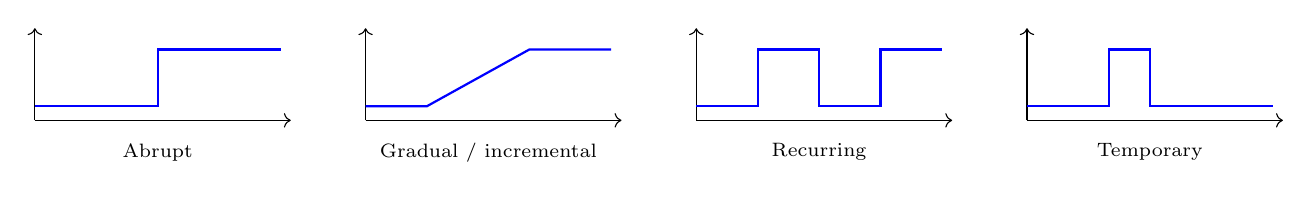
\begin{tikzpicture}[x=0.26cm,y=0.9cm,font=\scriptsize]
  % abrupt
  \begin{scope}
    \draw[->] (0,0) -- (12.5,0); \draw[->] (0,0) -- (0,1.3);
    \draw[thick,blue] (0,0.2) -- (6,0.2) -- (6,1.0) -- (12,1.0);
    \node at (6,-0.45) {Abrupt};
  \end{scope}
  \begin{scope}[xshift=4.2cm]
    \draw[->] (0,0) -- (12.5,0); \draw[->] (0,0) -- (0,1.3);
    \draw[thick,blue] (0,0.2) -- (3,0.2) -- (8,1.0) -- (12,1.0);
    \node at (6,-0.45) {Gradual / incremental};
  \end{scope}
  \begin{scope}[xshift=8.4cm]
    \draw[->] (0,0) -- (12.5,0); \draw[->] (0,0) -- (0,1.3);
    \draw[thick,blue] (0,0.2) -- (3,0.2) -- (3,1.0) -- (6,1.0) -- (6,0.2) -- (9,0.2) -- (9,1.0) -- (12,1.0);
    \node at (6,-0.45) {Recurring};
  \end{scope}
  \begin{scope}[xshift=12.6cm]
    \draw[->] (0,0) -- (12.5,0); \draw[->] (0,0) -- (0,1.3);
    \draw[thick,blue] (0,0.2) -- (4,0.2) -- (4,1.0) -- (6,1.0) -- (6,0.2) -- (12,0.2);
    \node at (6,-0.45) {Temporary};
  \end{scope}
\end{tikzpicture}
\caption{Shapes of concept drift: the vertical axis is the degree of change in traffic behaviour relative to the training data and the horizontal axis is time.}
\label{fig:drifttypes}
\end{figure}

The common response to drift is retraining. Retraining has a cost in computing time and validation effort, and it carries a risk: a model retrained only on recent data can forget older attacks that are still relevant (catastrophic forgetting), and a badly retrained model can be worse than the one it replaces. Recent research on continual-learning IDS, discussed in Chapter~2, shows good mechanisms for adapting a model. However, those mechanisms are usually applied in one fixed way whenever drift is flagged, and the updated model is usually put straight into service.

This project proposes \textbf{EVO-X}, a framework that treats the evolution of a deployed IDS as a governed decision process instead of an automatic reflex. Figure~\ref{fig:conceptual} contrasts the conventional approach with the EVO-X approach. In EVO-X, drift is detected and characterised, a controller chooses one of five adaptation strategies, the strategy produces a \emph{candidate} model that is never deployed directly, the candidate is tested on independent recent and historical data, a safety gate approves or rejects it, and an approved model is monitored after deployment and rolled back if it degrades. The classifier itself (a Random Forest or XGBoost model working on network-flow features) is a replaceable component and is not the contribution of the project; the contribution is the governance layer around it.

\begin{figure}[h]
\centering
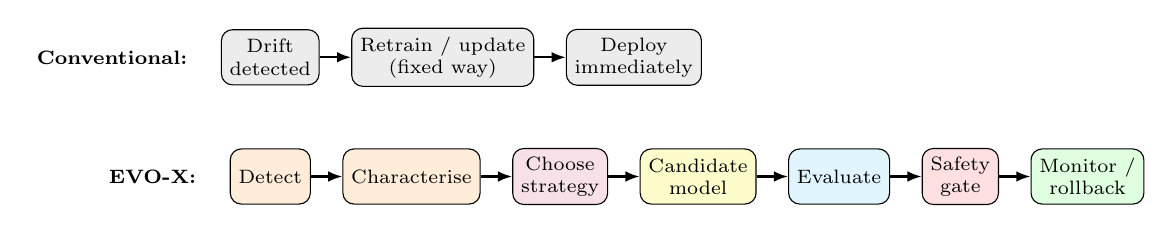
\begin{tikzpicture}[node distance=3mm and 4mm,
  box/.style={draw,rounded corners,align=center,minimum height=7mm,font=\scriptsize,inner sep=3pt},
  arr/.style={-{Latex[length=1.8mm]},thick}]
  \node[box,fill=gray!15] (a1) {Drift\\detected};
  \node[box,fill=gray!15,right=of a1] (a2) {Retrain / update\\(fixed way)};
  \node[box,fill=gray!15,right=of a2] (a3) {Deploy\\immediately};
  \draw[arr] (a1)--(a2); \draw[arr] (a2)--(a3);
  \node[left=3mm of a1,font=\scriptsize\bfseries,align=right] {Conventional:};
  \node[box,fill=orange!15,below=8mm of a1] (b1) {Detect};
  \node[box,fill=orange!15,right=of b1] (b2) {Characterise};
  \node[box,fill=purple!12,right=of b2] (b3) {Choose\\strategy};
  \node[box,fill=yellow!20,right=of b3] (b4) {Candidate\\model};
  \node[box,fill=cyan!12,right=of b4] (b5) {Evaluate};
  \node[box,fill=red!12,right=of b5] (b6) {Safety\\gate};
  \node[box,fill=green!12,right=of b6] (b7) {Monitor /\\rollback};
  \foreach \i/\j in {b1/b2,b2/b3,b3/b4,b4/b5,b5/b6,b6/b7}{\draw[arr] (\i)--(\j);}
  \node[left=3mm of b1,font=\scriptsize\bfseries,align=right] {EVO-X:};
\end{tikzpicture}
\caption{Conventional ``drift detected, so retrain'' reflex versus the governed evolution loop of EVO-X.}
\label{fig:conceptual}
\end{figure}

\subsection{Problem Statement}

Static machine-learning IDS models degrade when network traffic evolves, because concept drift introduces new attack patterns and changes normal behaviour. Periodic retraining is expensive and can cause catastrophic forgetting of previously learned attacks. Existing adaptive IDS apply a fixed adaptation strategy once drift is detected, without considering the type, severity or persistence of the drift, and they often lack a safety mechanism to validate an updated model before deployment. The problem addressed here is to design and evaluate an autonomous IDS that detects, characterises and responds to concept drift by selecting a suitable adaptation strategy and promoting an updated model only if it is demonstrably safe.

The problem is hard for several reasons. Drift must be detected from signals that are partly unavailable at run time, because true labels arrive late or not at all. Different drifts call for different responses: a brief blip should be ignored, a recurring pattern can be handled with memory of the past, and a new attack family may need a fresh model. Updates must balance plasticity (learning the new) against stability (keeping the old), and the quality of an update can be judged only on data that the update did not train on. In terms of the state of the art, mechanisms for drift detection and continual learning are well developed, while the orchestration of several adaptation options with an explicit candidate safety gate and rollback is comparatively less studied for network-flow IDS.

\subsection{Motivation}

The motivation for this project has three parts. First, \emph{operational realism}: in real security operations a deployed model is not retrained blindly on every new batch of data, because retraining costs compute, downtime and validation effort and a bad retraining can make things worse. Mature machine-learning operations (MLOps) practice already manages other production models with versioning, validation before release and rollback, but this discipline is largely absent from the academic continual-learning IDS literature.

Second, \emph{forgetting is a safety risk}. An IDS that adapts to new attacks but forgets older, still-relevant ones may be more dangerous than one that does not adapt at all, because operators may believe protection has improved when it has not. A framework that explicitly measures and gates against forgetting addresses a practical blind spot. Third, the project has \emph{educational and research value}: it requires concept-drift theory, continual learning, multi-objective decision making, streaming systems and model lifecycle practice together, at a depth appropriate for a final-year research project that a small team can complete in one academic year.

The people who should care about this work are security operations teams who run learning-based detectors, researchers in adaptive and continual-learning IDS, and engineers responsible for keeping production machine-learning models safe and auditable.

\subsection{Significance of the problem}

The approach of EVO-X is to separate the question \emph{how to adapt} from the question \emph{whether and which adaptation to apply}. The hypothesis behind the design is that choosing the adaptation according to the measured nature of the drift, and refusing to deploy any update that fails an independent check, will give fewer unnecessary and fewer harmful updates than always applying the same update, at comparable detection quality. Existing systems are not adequate for this purpose because, as Chapter~2 explains, they provide strong update mechanisms but a single fixed pipeline and little or no candidate validation. EVO-X is not claimed to invent drift detection or continual learning; the novel element is the combination of multi-strategy selection, independent candidate evaluation, a fail-closed safety gate and monitored rollback for network-flow IDS.

The performance study streams real CICIDS2017 flows with controlled, injected drift of six types (abrupt, gradual, recurring, temporary, incremental and novel-class) and a drift-free control, and compares ten policies: a static model, four fixed update policies, one SSF-inspired policy, an active-learning-inspired policy, EVO-X and three EVO-X ablations. The measured quantities include macro-averaged F1, historical forgetting, false-positive change, number of updates, training and proxy-search time, and counts of harmful and unnecessary updates. The first quick run on real flows (seven scenarios, one test seed) shows that updating is not automatically beneficial: some fixed-update policies improved macro-F1 over the static model by up to about four points while others lowered it and caused much more forgetting, and EVO-X, which made no promotions in this run, matched the static model without forgetting but showed no gain. The hypotheses are therefore inconclusive at this stage, and the report states this plainly. The full multi-seed experiment is the remaining step needed to decide them.

	\pagebreak

	\section{Literature Review , Gap Identified}

This chapter first gives the background needed to understand the work and then reviews related systems, ending with the gap that EVO-X targets.

\subsection{Background}

\textbf{Flow-based IDS.} A network flow summarises a conversation between two hosts, for example by its duration, packet and byte counts, inter-arrival times and flag counts. Flow-based IDS classify each flow, which keeps the input small and independent of packet payloads. CICIDS2017 \cite{sharafaldin2018cicids} provides labelled flows for benign traffic and attacks such as DoS, DDoS, brute force, infiltration, botnet and web attacks; UNSW-NB15 \cite{moustafa2015unsw} and CSE-CIC-IDS2018 \cite{cse2018} offer different feature sets and attack families. These benchmarks are widely used but are known to contain labelling and generation artefacts, so results on them are best read as comparisons between methods rather than as absolute real-world performance.

\textbf{Concept drift.} Gama et al.\ \cite{gama2014survey} survey concept-drift adaptation, define the abrupt, gradual, incremental and recurring types, and separate \emph{detect-and-adapt} strategies from continuous adaptation. Drift can affect the input distribution (covariate shift), the class priors (prior shift) or the relation between features and labels. Detection can use the model's error stream, which needs labels, or can compare feature distributions, which does not.

\textbf{Drift detectors used in this project.} ADWIN \cite{bifet2007adwin} keeps a variable-length window over a stream and shrinks it when two sub-windows have significantly different means; it carries a theoretical bound on false positives. The Page--Hinkley test \cite{page1954ph} accumulates deviations from the running mean and signals a sustained increase; it is light and suits abrupt change. The Population Stability Index (PSI) compares the distribution of each feature in a recent window against reference bins; by convention, values above 0.1 indicate moderate and above 0.25 major shift. Maximum Mean Discrepancy (MMD) \cite{gretton2012mmd} is a kernel two-sample statistic that can reveal multivariate changes, such as a change in correlation, that per-feature comparisons miss.

\textbf{Continual learning and forgetting.} Wang et al.\ \cite{wang2024cl} describe continual learning as a stability--plasticity trade-off: a model must stay plastic enough to learn new concepts yet stable enough not to forget old ones. Catastrophic forgetting means a sharp loss of performance on earlier classes after training on new data. Common mitigation families are replay (mixing remembered samples into training), regularisation and architectural methods.

\subsection{Related Work}

\textbf{Surveys.} A 2024 survey on concept drift and feature dynamics in intrusion detection \cite{evolving2024survey} confirms that cybersecurity environments change in ways static IDS struggle with and catalogues detection and adaptation techniques; it informed the design of the drift-detection module.

\textbf{SSF.} Zhang et al.\ \cite{zhang2024ssf} propose a continual-learning method for network IDS that combines drift detection, a strategic sample-selection step that prioritises samples showing the drifted pattern, a strategic forgetting step that discards outdated buffered samples when significant drift is seen, and periodic fine-tuning. It reports state-of-the-art adaptability on NSL-KDD and UNSW-NB15. Its strength is a well-designed adaptation mechanism; its limitation for our purposes is that the same pipeline is applied whenever drift is detected.

\textbf{RepShield.} Liu et al.\ \cite{liu2026repshield} address forgetting at the optimisation level: a historical feature subspace is built using PCA-based drift detection and new gradient updates are projected onto its orthogonal complement, so new learning interferes less with old knowledge. It also uses strategic sample selection. Again the mechanism is fixed rather than one option among several.

\textbf{METANOIA.} Ying et al.\ \cite{ying2025metanoia} present a lifelong provenance-based intrusion detection and investigation system for host-level attacks such as advanced persistent threats. It treats lifelong operation as a system-design concern, which is closest in spirit to this project, but it targets host and provenance data instead of network flows and has no explicit multi-strategy controller or candidate promotion gate.

\textbf{Deciding when to retrain.} Pham et al.\ \cite{pham2025retrain} study when a deployed ML system should be retrained and propose a semi-supervised drift-detection technique that reduces labelling effort. This frames retraining as a deliberate decision, in the same spirit as EVO-X, but it is not specific to IDS and does not choose among adaptation types or validate candidates.

\textbf{Online and active learning.} The project proposal also cites a drift-aware hybrid online IDS that combines drift detection with online and active learning to reduce unnecessary labelling and retraining. The exact bibliographic reference could not be verified, so the report describes the corresponding baseline by its mechanism (incremental learning on the least-confident labelled samples) and does not cite it by name. \todo{replace with the verified citation or keep as is}

\begin{table}[h]
\centering
\caption{Summary of what existing work demonstrates and what is left open.}
\label{tab:related}
\small
\begin{tabular}{p{2.6cm}p{5.2cm}p{5.4cm}}
\toprule
System & Demonstrated & Left open (relative to this project) \\
\midrule
SSF \cite{zhang2024ssf} & Strategic selection and forgetting in one pipeline & One fixed strategy; no candidate gate \\
RepShield \cite{liu2026repshield} & Gradient projection against forgetting & One fixed mechanism; no strategy choice \\
METANOIA \cite{ying2025metanoia} & Lifelong host-level APT detection & Not network-flow; no controller or gate \\
Pham et al.\ \cite{pham2025retrain} & Deciding when to retrain & Not IDS-specific; no strategy choice or safety check \\
\bottomrule
\end{tabular}
\end{table}

\subsection{Gap Identified}

It would be wrong to say that no adaptive IDS exists; SSF, RepShield and METANOIA show working adaptive systems, and drift detection and continual learning are established fields. What appears comparatively under-explored for network-flow IDS is a management layer that (i) chooses among qualitatively different adaptation strategies according to the measured characteristics of the drift, (ii) treats the trade-off between performance gain, forgetting, cost and false-positive risk as an explicit multi-objective decision, (iii) evaluates every adaptation as a candidate on both recent and historical data before deployment, (iv) keeps a versioned lifecycle with automatic rollback, and (v) is evaluated for portability across more than one classifier and more than one dataset. This gap has to be re-verified against the newest literature at the time of final submission, because the area moves quickly. \todo{record the date and search terms of the final literature check}

EVO-X is better suited to this gap than the reviewed systems because it keeps their adaptation mechanisms as options (incremental learning, replay, strategic sample selection, full retraining), adds a transparent controller whose every decision is logged, and refuses to deploy a candidate that fails an independent check. Where its contribution overlaps existing work, for instance METANOIA's lifelong-operation framing or general MLOps rollback patterns, the overlap is acknowledged, and the claim is limited to the specific combination applied to network-flow IDS.

    \pagebreak
    \section{Customer Details and Use Cases}

This chapter records the external expert consulted during the project and describes the situations in which the system is meant to be used.

\subsection{Customer Details}

\begin{table}[h]
\centering
\caption{Customer / expert-consultation details.}
\small
\begin{tabular}{p{3.5cm}p{9cm}}
\toprule
Customer name & Anish Shobith P S \\
Contact person & Anish Shobith P S, Master's student (Cyber Security), Manipal School of Information Sciences \\
Contact & Website: https://anishshobithps.com/; LinkedIn: linkedin.com/in/anishshobithps/; Email: anish.shobith19@gmail.com \\
Nature of engagement & Research-oriented academic consultation, contacted through LinkedIn to review the project synopsis and suggest improvements to the research direction and methodology \\
\bottomrule
\end{tabular}
\end{table}

\subsection{Feedback Received and How It Was Addressed}

After reading the synopsis, the reviewer said that the orchestration layer, in which drift analysis, multi-strategy adaptation and a pre-deployment safety gate sit in one loop, was the most interesting part, and he pushed on specific points. The visible points of his message and the corresponding project actions are summarised in Table~\ref{tab:feedback}. \todo{the screenshot shows three of the four points; add the fourth point and its response from the original message}

\begin{table}[h]
\centering
\caption{Expert feedback and corresponding action.}
\label{tab:feedback}
\small
\begin{tabular}{p{5.4cm}p{7.6cm}}
\toprule
Feedback & Action taken \\
\midrule
The selection logic of the Evolution Controller must be spelled out, since it is the core and the least specified part. & The controller was specified as eligibility rules plus utility ranking, with every decision logged (Sections 5.2 and 5.4). \\
Utility-function weights should come out of experiments instead of being asserted, showing what happens when they move. & Weights and gate thresholds are selected on validation scenarios only from predeclared grids, frozen before testing, and the sensitivity grids are reported. \\
Benchmark against SSF and HOIDS; a softer comparison will not say much. & An SSF-inspired baseline and an active-learning-inspired baseline are included among ten compared policies. \\
\bottomrule
\end{tabular}
\end{table}

\subsection{Use Cases}

The system is intended for the following situations; the use-case diagram is in Section 5.4.2.

\begin{enumerate}
\item \textbf{SOC engineer keeps a learned detector current.} A security operations team that runs a flow-based ML detector wants it to adapt to new traffic without constant manual retraining, while being confident that no update silently weakens protection. EVO-X proposes updates, validates them and records why each decision was taken.
\item \textbf{Researcher compares adaptation policies.} An IDS researcher can plug a new adaptation strategy, drift detector or classifier into the framework and compare it against the fixed policies under the same scenarios, label policy and statistics.
\item \textbf{Operator audits model changes.} A reviewer can inspect the evolution history: which drift triggered an update, what the controller chose and why, how the candidate scored, whether the gate promoted it and whether a rollback happened.
\item \textbf{Safe experimentation.} A team that wants to try a more aggressive update can run it through the gate and the post-deployment monitor, so that a harmful change is rejected or reverted instead of reaching production.
\end{enumerate}

\pagebreak
\section{Project Objectives}

\begin{enumerate}
\item To build a streaming evaluation environment that replays benchmark intrusion data in time order and injects controlled drift of six types.
\item To detect and characterise concept drift using ADWIN, Page--Hinkley, PSI and MMD, individually and in fusion, and to summarise each drift by its magnitude, persistence, unfamiliarity and recurrence.
\item To design an Evolution Controller that selects among no-op, incremental learning, memory replay, strategic sample selection and full retraining.
\item To evaluate every candidate model on independent recent and historical data and to promote it only through a safety gate with versioned registry and automatic rollback.
\item To compare EVO-X experimentally against static and fixed-strategy baselines using predeclared statistics and to report the outcome honestly, including where it does not help.
\end{enumerate}

\pagebreak
	\section{Proposed Method/Algorithm }

This chapter restates the problem formally, describes the idea of EVO-X and its architecture with a worked example, and presents the analysis and design of the system.

	\subsection{Problem Definition}

\textbf{Inputs.} (i) A stream of time-ordered batches $B_1,B_2,\dots$ of network flows, each flow described by a numeric feature vector $x$ and carrying a class label $y$ (benign or an attack family); labels of batch $t$ become available only after a delay of $k$ batches. (ii) An initial deployed model $M_1$ trained on a reference window. (iii) Role-separated data for evaluation: proxy, gate, monitor and reporting holdouts. (iv) A set of adaptation strategies $\mathcal{A}=\{\text{No-Op},\text{Incremental},\text{Replay},\text{Strategic},\text{Retrain}\}$ and resource budgets for training time and latency.

\textbf{Outputs.} A sequence of deployed model versions $M_v$, together with a log recording for every drift event the drift signature, the chosen strategy, the candidate's evaluation, the gate decision and any rollback.

\textbf{Objective.} Keep the predictive quality of the deployed model high on both recent and historical traffic over the whole stream while performing few updates, spending little adaptation cost and never promoting a harmful candidate. For a policy $\pi$ that produces the model $M^{\pi}_t$ deployed at time $t$ this can be written as
\begin{equation}
\max_{\pi}\; \frac{1}{T}\sum_{t=1}^{T}\tfrac12\big(F1^{\text{recent}}_t(M^{\pi}_t)+F1^{\text{hist}}_t(M^{\pi}_t)\big)\;-\;\lambda\,\text{Cost}(\pi),
\end{equation}
subject to the promotion constraints of the safety gate given in Section 5.4.4.

\textbf{Constraints.} Labels arrive late and may be partial; a candidate must be judged only on data it was not trained on; training time and inference latency must stay within budget; the active model must remain unchanged if any check fails.

\textbf{Assumptions.} Labels eventually become available for adaptation; the monitored signals (error rate, feature distributions) reflect real changes in traffic; the holdout data are representative of recent and historical traffic; experiments replay public benchmarks, not live networks.

\textbf{Key challenges.} Detecting drift without immediate labels; distinguishing temporary blips from lasting change; balancing plasticity against forgetting; estimating the value of an update cheaply before paying for it; avoiding leakage between training and evaluation data; and choosing thresholds and weights without tuning them on the test data.

	\subsection{Proposed Idea/System}

EVO-X replaces ``drift detected $\rightarrow$ retrain'' with a decision-and-evaluation pipeline of seven cooperating stages. \emph{Detection} produces an alarm; \emph{analysis} turns it into a drift signature; the \emph{controller} selects a strategy; the \emph{adaptation engine} builds a candidate; \emph{evaluation} scores the candidate on independent holdouts; the \emph{safety gate} promotes or rejects it; and \emph{lifecycle management} versions, monitors and, if needed, rolls back the model. The underlying classifier is a replaceable component. The ideas that are new compared with the reviewed work are: the explicit, logged two-stage choice among several adaptation strategies; the rule that a candidate is never deployed before an independent check; the fail-closed behaviour of the gate; and the tamper-evident versioning with monitored rollback, all applied to network-flow IDS.

	\subsection{System Architecture}

Figure~\ref{fig:architecture} shows the end-to-end architecture. Data from the benchmark datasets and the synthetic drift generator are streamed in time order through a preprocessing stage to the currently deployed IDS. The drift engine monitors the stream and hands alarms to the drift analyzer; the Evolution Controller picks a strategy; the adaptation engine produces a candidate; the evaluator scores it; the safety gate decides; and the registry and evolution history record everything. A dashed feedback path lets stored drift signatures support recurrence matching.

\begin{figure}[p]
\centering
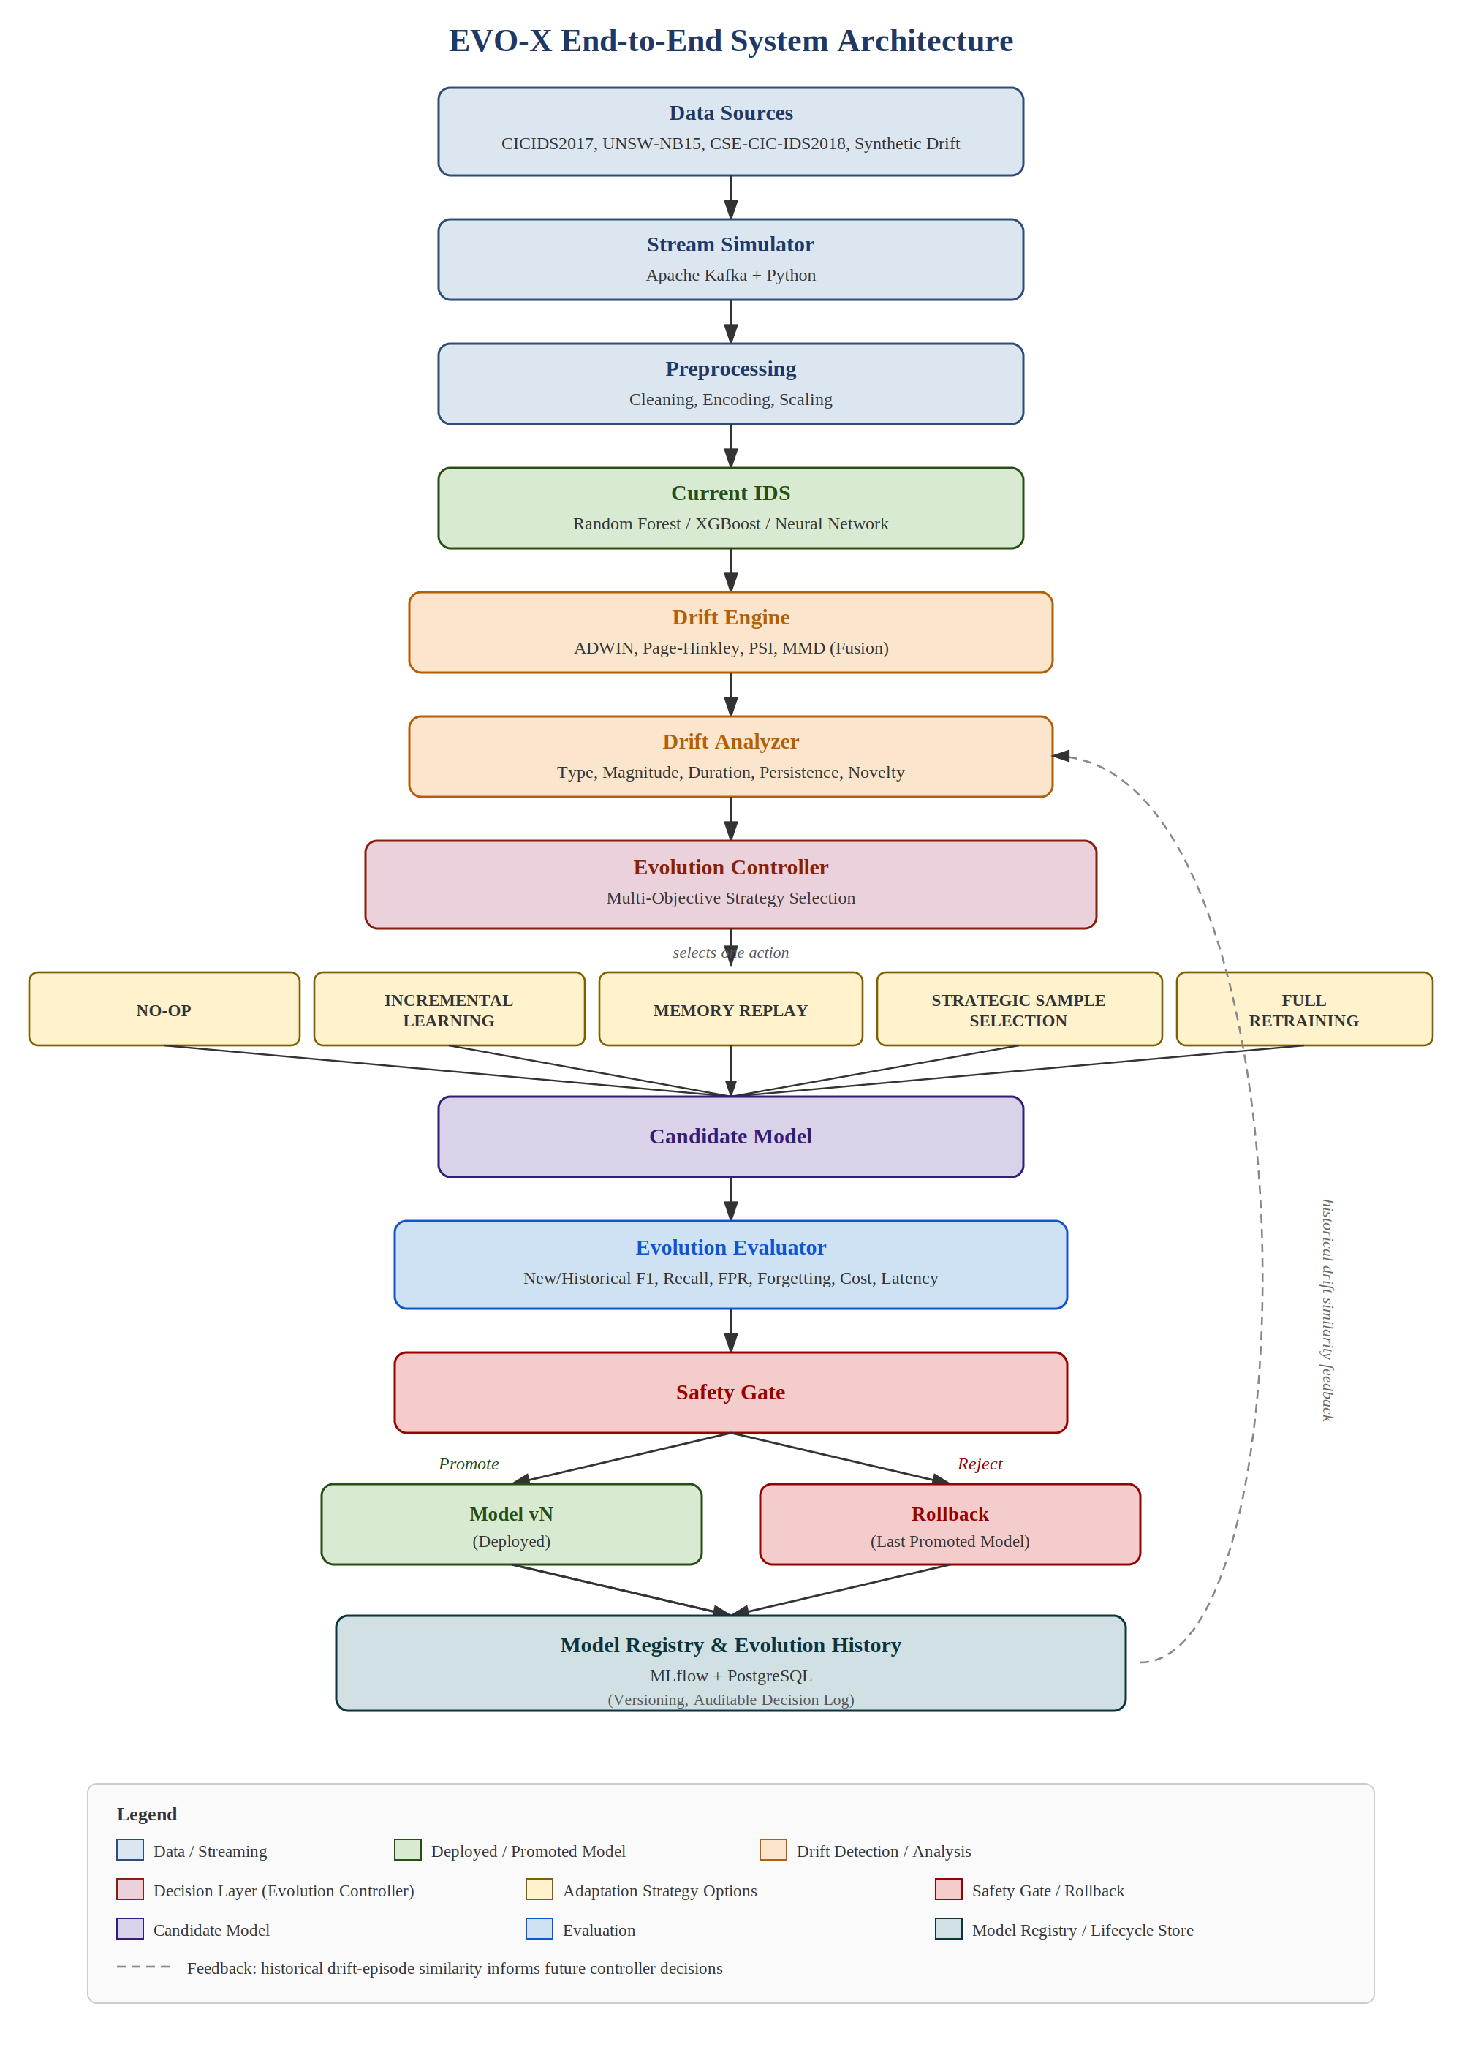
\includegraphics[height=0.80\textheight]{figs/architecture.png}
\caption{End-to-end architecture of EVO-X.}
\label{fig:architecture}
\end{figure}

\textbf{Drift detection.} ADWIN monitors the per-flow error bits and Page--Hinkley monitors the per-batch error rate; both see labels only after the label delay. The PSI detector compares a sliding window of the last few batches with the reference using ten reference-quantile bins per feature and aggregates the per-feature values as the mean of the five largest, so that a shift in a few features is not diluted by many unchanged ones. The MMD detector uses a Gaussian (RBF) kernel with the median-distance bandwidth on subsamples; its alarm threshold is calibrated from windows drawn from a disjoint half of the reference data. An extra label-free signal applies ADWIN to the prediction confidence. Each detector reports a score normalised so that 1.0 is its own alarm threshold, and the scores are fused:
\begin{equation}
D_{\text{fused}}=\sum_i w_i\,\min(s_i,1),\qquad \sum_i w_i=1,
\label{eq:fusion}
\end{equation}
with an alarm on the rising edge of $D_{\text{fused}}\ge\theta$ and a re-arming rule so that one drift gives one alarm. PSI for one feature is $\sum_b (p_b^{\text{window}}-p_b^{\text{ref}})\ln\!\big(p_b^{\text{window}}/p_b^{\text{ref}}\big)$ over bins $b$, and the unbiased squared MMD between samples $X$ and $Y$ is $\text{MMD}^2=\tfrac{1}{n(n-1)}\sum_{i\ne j}k(x_i,x_j)+\tfrac{1}{m(m-1)}\sum_{i\ne j}k(y_i,y_j)-\tfrac{2}{nm}\sum_{i,j}k(x_i,y_j)$.

\textbf{Drift analysis.} For each alarm the analyzer waits a few batches, never looking beyond its observation point, and builds a \emph{drift signature}: magnitude (the mean of the PSI and MMD scores in units of their own thresholds), persistence (the longest run of batches above threshold), duration, an ``ended'' flag showing that the shift has already disappeared, a type guess (abrupt, gradual, temporary or recurring), a confidence-based unfamiliarity score, the per-feature PSI vector, and a recurrence score given by the cosine similarity of that vector with stored past signatures. The unfamiliarity score is only a hint: development tests showed that it also rises under plain covariate shift, so it never selects an action on its own.

\textbf{Adaptation strategies.} \emph{No-Op} returns the parent model unchanged. \emph{Incremental} updates the model with recent data: for Random Forest \cite{breiman2001rf} by pruning part of the ensemble and growing new trees, for XGBoost \cite{chen2016xgboost} by continuing boosting, which is available only if the set of classes has not changed. \emph{Replay} trains on recent data mixed with a bounded, class-balanced memory of earlier data. \emph{Strategic Selection} is inspired by SSF and keeps the samples with the largest error and lowest confidence, keeps every class represented and expires stale memory. \emph{Full Retrain} trains from scratch on recent data only. Every strategy produces a candidate that records its parent version, strategy, a hash of its training snapshot and its measured resource use; none of them changes the active model.

\textbf{Evolution controller.} Selection is done in two stages. Stage one applies eligibility rules (Algorithm~\ref{alg:rules}) to the signature, shrinking the five strategies to an admissible set; No-Op is always admissible. Stage two ranks the admissible set by a weighted utility,
\begin{align}
U(a)&=w_1\,\widehat{\Delta F1}(a)-w_2\,\widehat{\text{Forg}}(a)-w_3\,\widehat{\text{Cost}}(a)-w_4\,\widehat{\Delta\text{FPR}}(a)-w_5\,\widehat{\text{Lat}}(a),\label{eq:utility}\\
a^{*}&=\argmax_{a\in E}\,U(a),
\end{align}
where the estimates of gain, forgetting and false-positive change come from a cheap proxy evaluation on a small holdout, and cost and latency come from measured per-strategy profiles. Ties are broken towards No-Op and then towards the cheaper action. Because $a^{*}$ is only a provisional choice, the candidate it yields is still subject to the full evaluation and the safety gate.

\textbf{Worked example (illustrative numbers, not measured).} Suppose an alarm gives a signature with magnitude $4.2$ (above $\tau_{\text{high}}=3$), persistence $12$ batches (above $\tau_{p,\text{long}}=10$), recurrence $0.3$ and no ``ended'' flag. The rules admit $E=\{\text{Retrain},\text{Replay},\text{No-Op}\}$. Take weights $w=(0.4,0.2,0.2,0.1,0.1)$ and normalised proxy estimates as in Table~\ref{tab:example}. The utilities are $U(\text{Retrain})=0.4(0.12)-0.2(0.10)-0.2(0.10)-0.1(0.01)-0.1(0.10)=-0.003$, $U(\text{Replay})=0.4(0.10)-0.2(0.02)-0.2(0.05)-0.1(0.005)-0.1(0.10)=+0.0155$ and $U(\text{No-Op})=0$, so Replay is selected and its candidate goes to evaluation. The example also shows a property that matters later: if the estimated gains were smaller, the cost terms would dominate and No-Op would win, so the scale of the terms and the weights decide how willing the controller is to update.

\begin{table}[h]
\centering
\caption{Illustrative proxy estimates for the worked example (invented for explanation only).}
\label{tab:example}
\small
\begin{tabular}{lccccc}
\toprule
Action & $\widehat{\Delta F1}$ & $\widehat{\text{Forg}}$ & $\widehat{\text{Cost}}$ & $\widehat{\Delta\text{FPR}}$ & $\widehat{\text{Lat}}$ \\
\midrule
Retrain & 0.12 & 0.10 & 0.10 & 0.010 & 0.10 \\
Replay  & 0.10 & 0.02 & 0.05 & 0.005 & 0.10 \\
No-Op   & 0 & 0 & 0 & 0 & 0 \\
\bottomrule
\end{tabular}
\end{table}

\textbf{Independent evaluation and data roles.} To avoid leakage, every original source flow is assigned to exactly one role, even if it appears several times in the stream under different drift offsets: 50\% training, 15\% proxy estimation, 15\% gate evaluation, 10\% post-deployment monitoring and 10\% final reporting (Figure~\ref{fig:roles}). Candidates never train on proxy, gate, monitor or reporting rows, and reporting rows influence nothing at run time; they are used only for the final metrics. Historical validation samples are split by class across the four evaluation roles.

\begin{figure}[h]
\centering
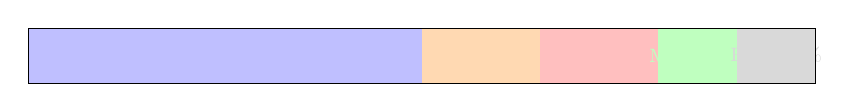
\begin{tikzpicture}[font=\scriptsize]
  \def\h{0.7}
  \fill[blue!25] (0,0) rectangle (5.0,\h) node[midway] {Training 50\%};
  \fill[orange!30] (5.0,0) rectangle (6.5,\h) node[midway] {Proxy 15\%};
  \fill[red!25] (6.5,0) rectangle (8.0,\h) node[midway] {Gate 15\%};
  \fill[green!25] (8.0,0) rectangle (9.0,\h) node[midway] {Mon.\ 10\%};
  \fill[gray!30] (9.0,0) rectangle (10.0,\h) node[midway] {Rep.\ 10\%};
  \draw (0,0) rectangle (10,\h);
\end{tikzpicture}
\caption{Role assignment of source flows. Each original flow belongs to exactly one role.}
\label{fig:roles}
\end{figure}

\textbf{Safety gate.} The gate promotes a candidate only if all six checks pass:
\begin{equation}
\Delta F1_{\text{new}}\ge\tau_1,\quad \Delta F1_{\text{hist}}\ge-\tau_2,\quad \text{Forg}\le\tau_3,\quad \Delta\text{FPR}\le\tau_4,\quad \text{Train}\le\tau_5,\quad \text{Lat}\le\tau_6 .
\label{eq:gate}
\end{equation}
A missing, non-finite or physically invalid metric causes rejection (fail-closed), and rejection leaves the active model unchanged. The thresholds are not guessed: they are selected from a predeclared grid of 48 configurations using validation scenarios and independent audit outcomes, and are frozen before test scenarios are built.

\textbf{Registry, monitoring and rollback.} Each policy owns a registry of versioned, checksum-verified model artifacts and an append-only, hash-chained journal of events (candidates, decisions, parameters, drift context and pointer changes). Replaying the journal reconstructs which version is deployed; a damaged journal makes the system fail closed. Versions move through the states CANDIDATE, DEPLOYED, SUPERSEDED, REJECTED and ROLLED\_BACK. After promotion the active model is replaced in one atomic step, and a monitor compares it with its frozen parent on fresh labelled rows and an independent historical anchor; if performance or false-positive rate degrades, the parent is restored. After the experiment, candidates and parents are also shadow-scored on ten future batches so that a promoted or rejected update can be classified as harmful (it would lower macro-F1 by more than 0.03) or unnecessary (its gain is below 0.01).

	\subsection{System Analysis and Design}

	\subsubsection{Requirement Specification}

The functional and non-functional requirements are listed in Tables~\ref{tab:fr} and \ref{tab:nfr}.

\begin{table}[h]
\centering
\caption{Functional requirements.}
\label{tab:fr}
\small
\begin{tabular}{p{1cm}p{11.8cm}}
\toprule
ID & Requirement \\
\midrule
FR1 & Replay benchmark flows as time-ordered batches through a producer/consumer pipeline whose predictions equal direct in-memory scoring. \\
FR2 & Generate six drift scenario types and a drift-free control with recorded ground truth, from disjoint validation and test pools. \\
FR3 & Detect drift with ADWIN, Page--Hinkley, PSI and MMD and fuse their scores. \\
FR4 & Produce a drift signature for each alarm without looking beyond the observation point. \\
FR5 & Select one of five strategies by eligibility rules and utility ranking and log every decision with its reasons. \\
FR6 & Generate candidate models that never replace the active model by themselves. \\
FR7 & Evaluate candidates on independent recent and historical holdouts. \\
FR8 & Apply a fail-closed safety gate with configurable thresholds. \\
FR9 & Version every model, keep a tamper-evident event journal, monitor promoted models and roll back on degradation. \\
FR10 & Compare ten policies under identical data, labels and alarms and report predeclared statistics. \\
\bottomrule
\end{tabular}
\end{table}

\begin{table}[h]
\centering
\caption{Non-functional requirements.}
\label{tab:nfr}
\small
\begin{tabular}{p{3.2cm}p{9.6cm}}
\toprule
Property & Requirement \\
\midrule
Reproducibility & Seeds, configurations, data hashes and thresholds are stored with each run; results can be regenerated. \\
Leakage control & Source-group data roles; test-family scenarios refused during tuning. \\
Auditability & Every promotion, rejection and rollback is recorded and the journal is hash-chained. \\
Safety & Any missing or invalid metric rejects a candidate; the active model is never modified by a rejection. \\
Portability & The classifier is replaceable (Random Forest, XGBoost) behind one interface; datasets enter through adapters. \\
Resource limits & Training under 30~s and inference under 100~ms per 1000 flows in the frozen configuration. \\
Honesty of reporting & Synthetic or quick runs are labelled and cannot feed final tables. \\
\bottomrule
\end{tabular}
\end{table}

	\subsubsection{Flowcharts / DFDs / UML / Functional Block Diagram}

Figure~\ref{fig:usecase} gives the use-case diagram: the operator or researcher views the dashboard and configures gate thresholds, while the automated Evolution Controller monitors traffic, detects and analyses drift, selects a strategy, generates and evaluates a candidate, promotes or rejects it and may roll back a version. Figure~\ref{fig:class} shows the main classes: the drift engine and analyzer produce a drift signature; the evolution controller selects an adaptation strategy (an abstract class with five concrete subclasses); a candidate model records its parent version; the evaluator scores candidates; the safety gate decides; and the model registry and evolution history store the outcome. Figure~\ref{fig:activity} is the activity diagram of one evolution cycle and Figure~\ref{fig:sequence} is the corresponding sequence diagram.

\begin{figure}[h]
\centering
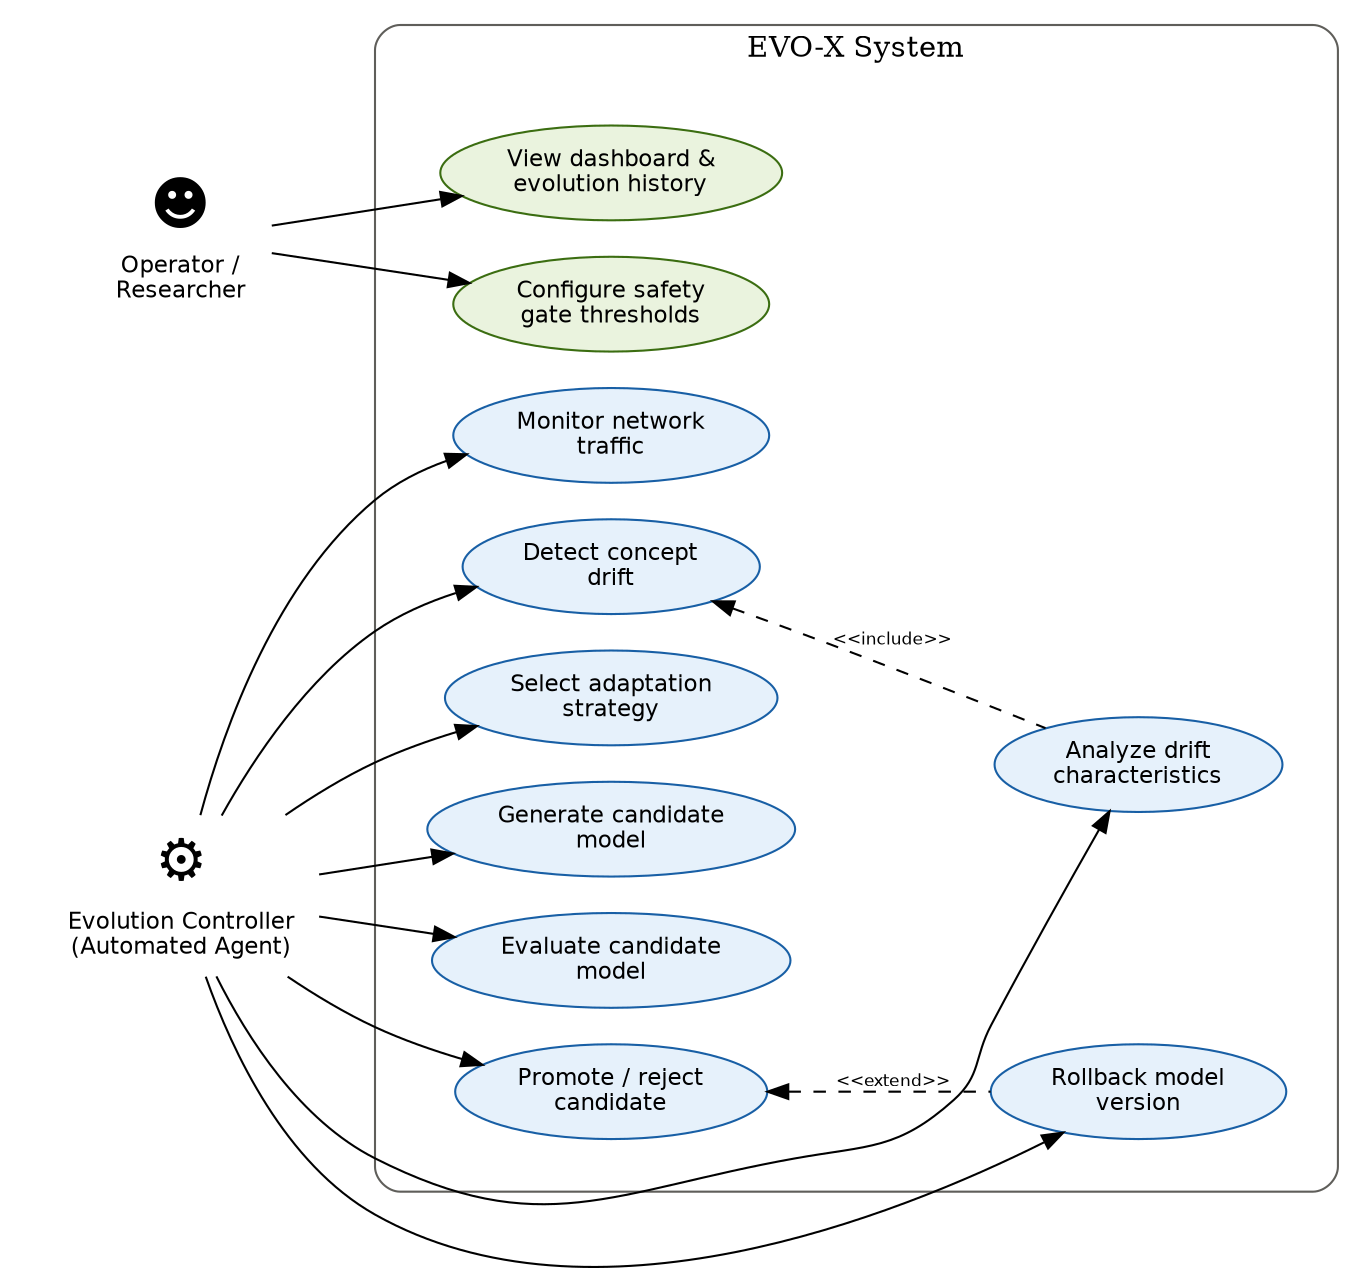
\includegraphics[width=0.78\textwidth]{figs/usecase.png}
\caption{Use-case diagram of EVO-X.}
\label{fig:usecase}
\end{figure}

\begin{figure}[h]
\centering
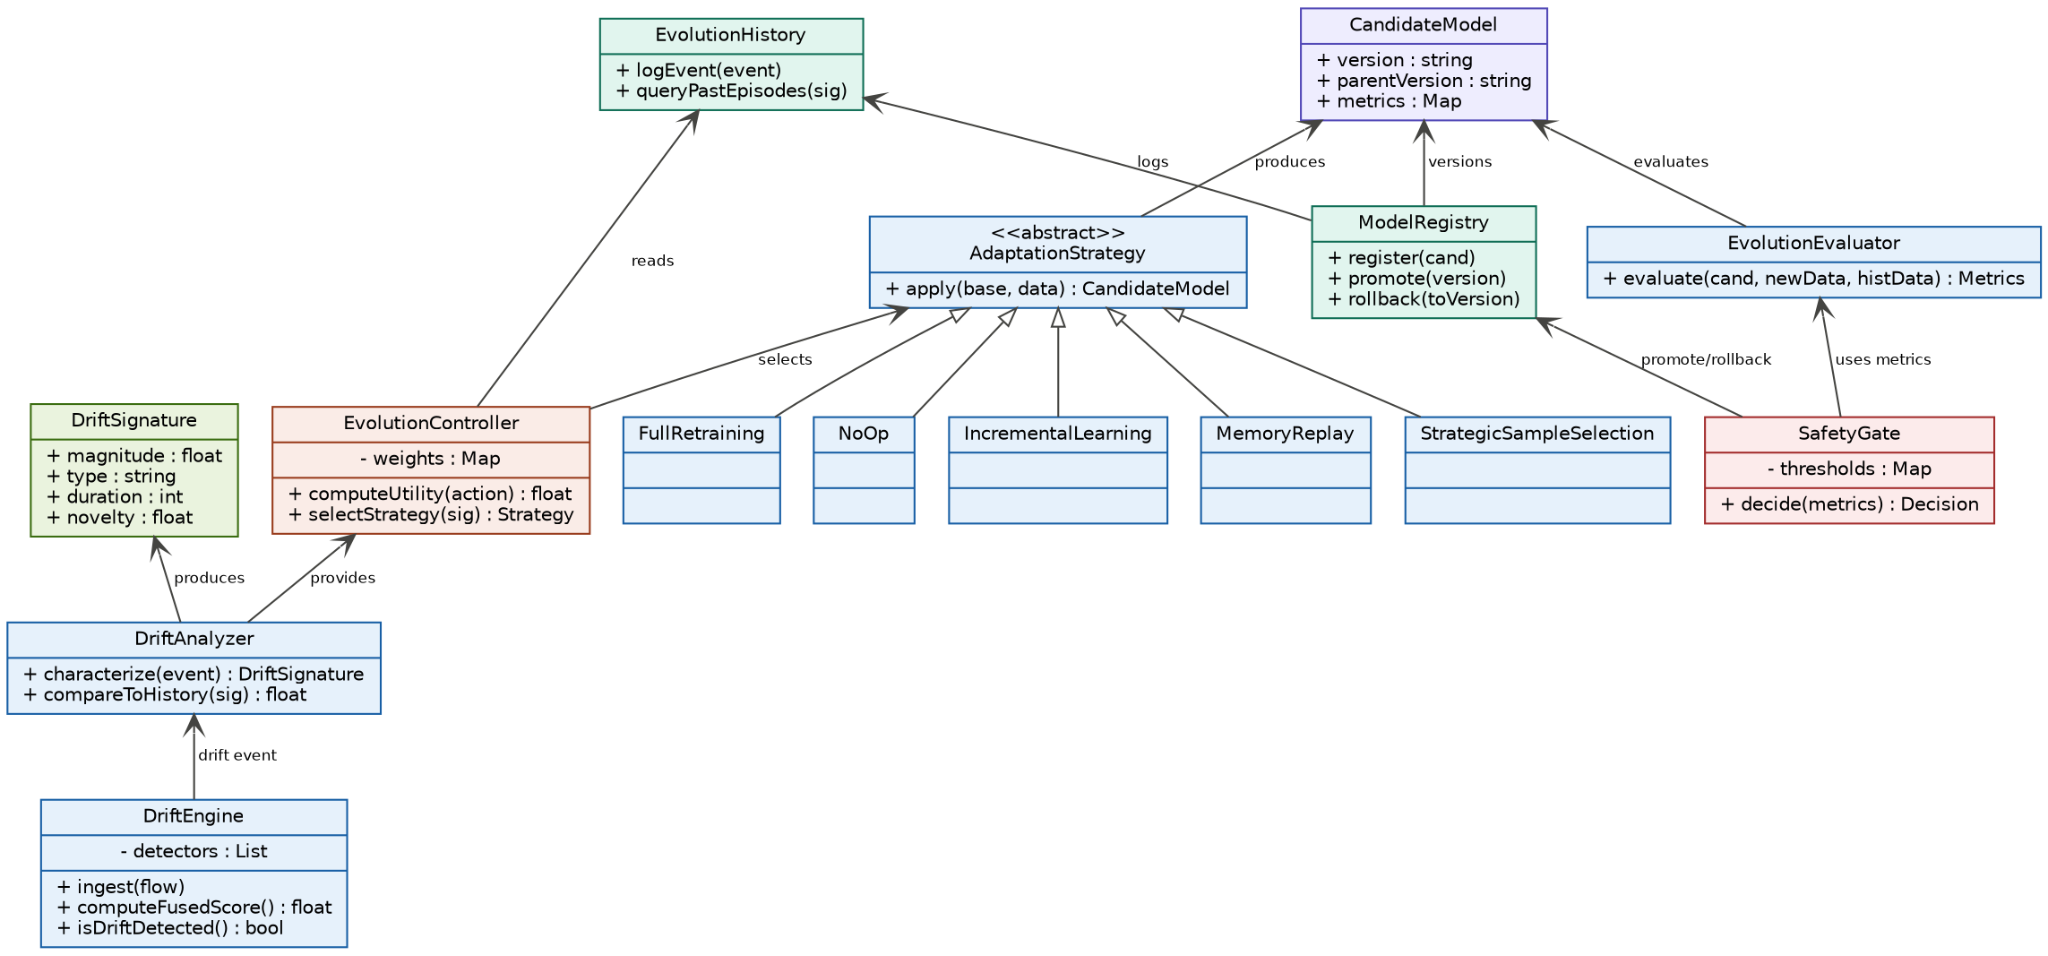
\includegraphics[width=\textwidth]{figs/classdiagram.png}
\caption{Class diagram of the main components.}
\label{fig:class}
\end{figure}

\begin{figure}[h]
\centering
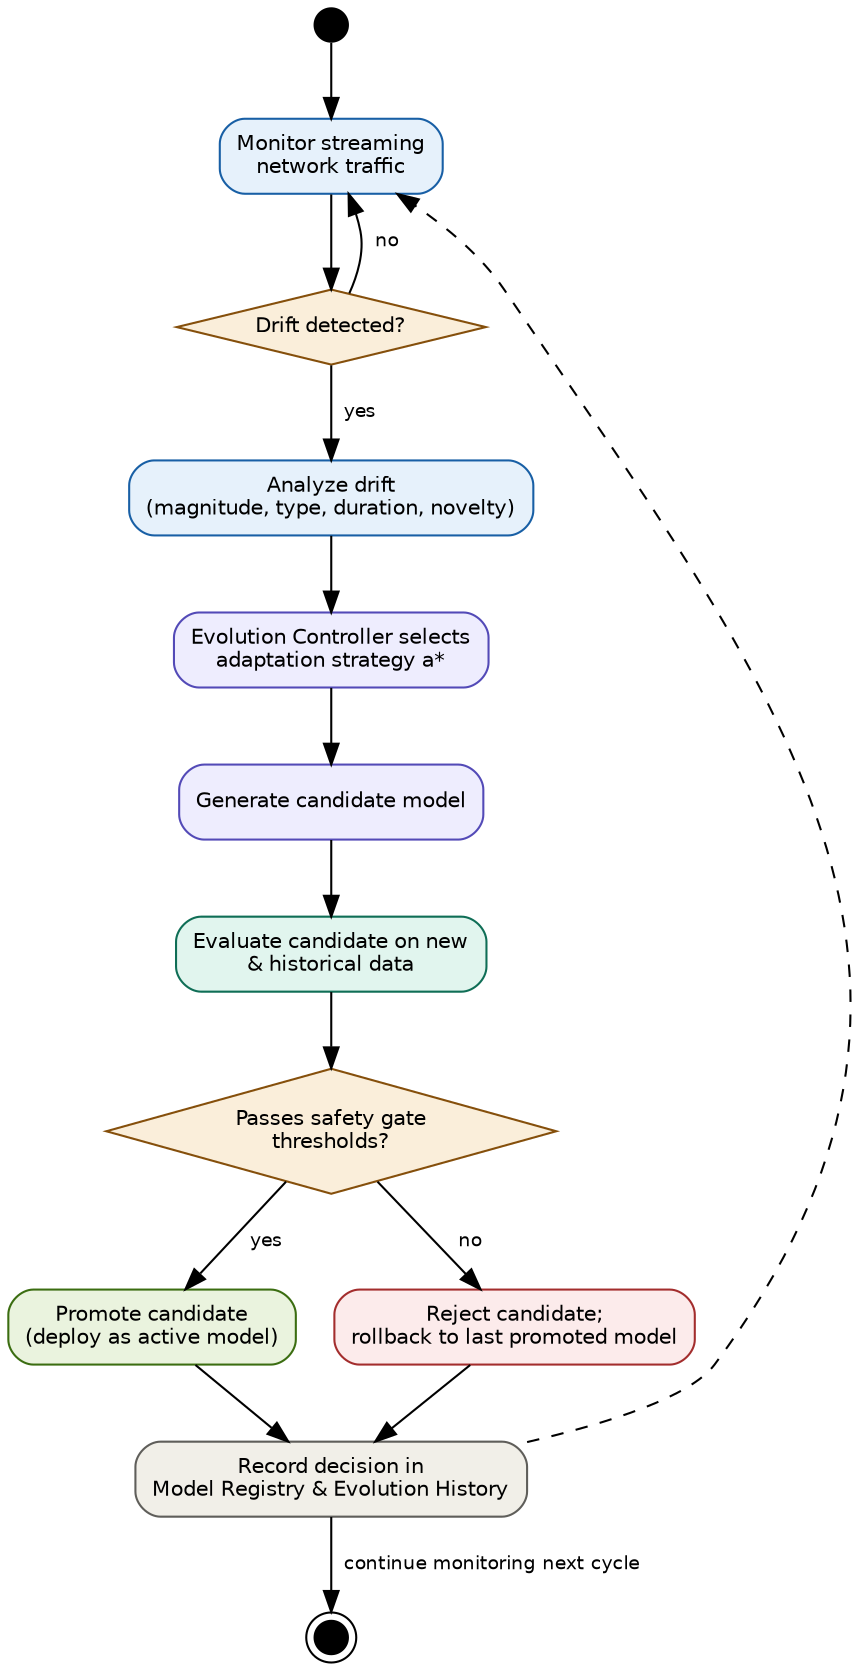
\includegraphics[height=0.72\textheight]{figs/activity.png}
\caption{Activity diagram of one evolution cycle.}
\label{fig:activity}
\end{figure}

\begin{figure}[h]
\centering
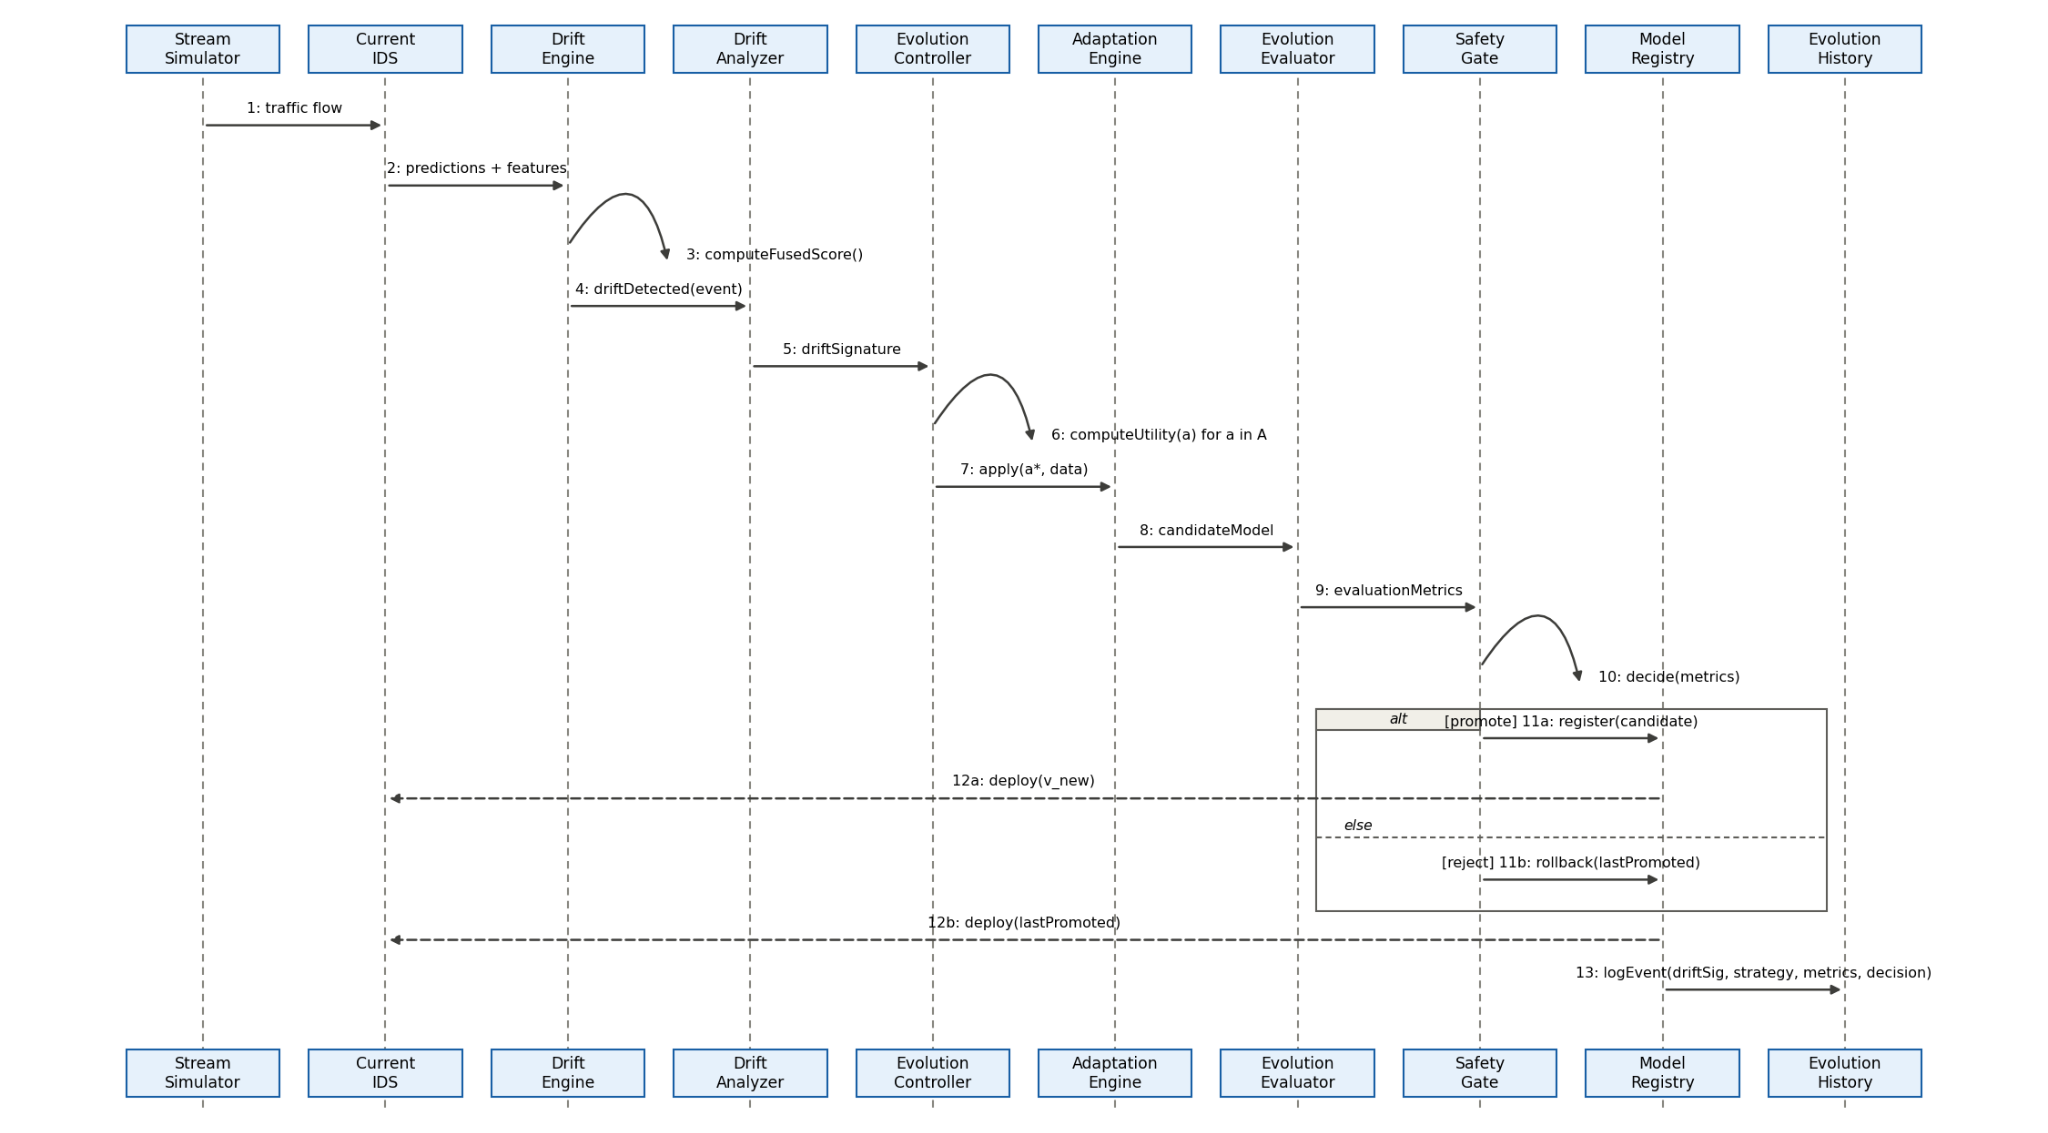
\includegraphics[width=\textwidth]{figs/sequence.png}
\caption{Sequence diagram of drift detection through promotion or rollback.}
\label{fig:sequence}
\end{figure}

	\subsubsection{Design and Test Cases}

Correctness of the mechanisms is verified by automated tests (207 tests in the Phase A--C implementation at the time of writing). The test cases most relevant to the design are listed in Table~\ref{tab:tests}. These tests show that the mechanisms behave as designed; they do not measure detection performance, which is the subject of Chapter~6.

\begin{table}[h]
\centering
\caption{Representative test cases.}
\label{tab:tests}
\small
\begin{tabular}{p{3.0cm}p{6.2cm}p{3.4cm}}
\toprule
Area & Test & Expected \\
\midrule
Streaming & Batch encoded, sent and decoded; delivery repeated; batch missing & Bit-identical data; duplicate skipped; gap raises error \\
Streaming & Scorer reads batch without labels & Labels never decoded \\
Streaming & Predictions through pipeline vs.\ direct loop & Identical predictions and confidences \\
Drift lab & Truth vs.\ generated stream; recurring segments; novel class first appearance & Truth matches data; recurrence repeats; first batch correct \\
Drift lab & Validation and test pools; magnitude levels & Pools disjoint; same drift at three strengths \\
Detectors & Step and ramp signals with known change point; stationary noise & Alarm shortly after change; few false alarms \\
Analyzer & Future data corrupted beyond observation point & Signature unchanged (no look-ahead) \\
Gate & Values exactly on and just beyond each threshold; missing metric & Boundary behaviour correct; reject on missing \\
Registry & Reject then promote then restore; reopen registry; damaged journal & Parent predictions restored exactly; state recovered; fail closed \\
Data roles & Source flow reused under different offsets & Stays in one role \\
\bottomrule
\end{tabular}
\end{table}

	\subsubsection{Algorithms and Pseudo Code}

Algorithm~\ref{alg:loop} is the main evolution loop, Algorithm~\ref{alg:rules} the eligibility rules and Algorithm~\ref{alg:gate} the safety gate.

\begin{algorithm}[h]
\caption{EVO-X evolution loop}
\label{alg:loop}
\small
\begin{algorithmic}[1]
\State deploy $M_1$; initialise registry, journal and signature store
\For{each batch $B_t$}
  \State predict $B_t$ with the deployed model; release labels of $B_{t-k}$
  \State update detectors; compute $D_{\text{fused}}$
  \If{alarm raised}
    \State wait for the observation window; $\sigma\gets$ \textsc{Characterise}(history up to now)
    \State $E\gets$ \textsc{Eligible}$(\sigma)$; $a^{*}\gets\arg\max_{a\in E}U(a)$
    \If{$a^{*}\ne$ No-Op}
      \State $M'\gets$ \textsc{Adapt}$(M_v,a^{*},\text{released labels})$
      \State metrics $\gets$ \textsc{Evaluate}$(M',M_v,\text{recent and historical holdouts})$
      \If{\textsc{Gate}(metrics) passes} \State promote $M'$ as new deployed version; start monitor
      \Else \State reject $M'$; keep $M_v$ \EndIf
    \EndIf
    \State append decision record to the journal
  \EndIf
  \If{monitor reports degradation} \State restore the parent version \EndIf
\EndFor
\end{algorithmic}
\end{algorithm}

\begin{algorithm}[h]
\caption{Eligibility rules (thresholds are parameters; implemented defaults in text)}
\label{alg:rules}
\small
\begin{algorithmic}[1]
\Require magnitude $m$, persistence $p$, ended flag, recurrence $r$, unfamiliarity $n$, budget
\If{$m<\tau_{\text{low}}$ \textbf{or} $p<\tau_{p,\text{short}}$ \textbf{or} ended} \State $E\gets\{\text{No-Op}\}$
\ElsIf{$r\ge\tau_{\text{rec}}$} \State $E\gets\{\text{Replay, Incremental, No-Op}\}$
\ElsIf{$n\ge\tau_{\text{nov}}$ \textbf{and} $m\ge\tau_{\text{high}}$} \State $E\gets\{\text{Retrain, Strategic, No-Op}\}$
\ElsIf{$m\ge\tau_{\text{high}}$ \textbf{and} $p\ge\tau_{p,\text{long}}$} \State $E\gets\{\text{Retrain, Replay, No-Op}\}$
\Else \State $E\gets\{\text{Incremental, Strategic, Replay, No-Op}\}$
\EndIf
\State remove unavailable actions and actions whose estimated cost exceeds the budget
\end{algorithmic}
\end{algorithm}
The implemented defaults are $\tau_{\text{low}}=1$, $\tau_{\text{high}}=3$, $\tau_{p,\text{short}}=2$, $\tau_{p,\text{long}}=10$, $\tau_{\text{rec}}=0.9$ and $\tau_{\text{nov}}=0.2$. \todo{confirm the values frozen for the final run}

\begin{algorithm}[h]
\caption{Safety gate (fail-closed)}
\label{alg:gate}
\small
\begin{algorithmic}[1]
\Require candidate metrics $\mu$, thresholds $\tau_1,\dots,\tau_6$
\If{any required metric is missing, non-finite or invalid} \State \Return \textsc{Reject}
\EndIf
\If{$\Delta F1_{\text{new}}\ge\tau_1$ \textbf{and} $\Delta F1_{\text{hist}}\ge-\tau_2$ \textbf{and} Forg$\le\tau_3$ \textbf{and} $\Delta$FPR$\le\tau_4$ \textbf{and} Train$\le\tau_5$ \textbf{and} Lat$\le\tau_6$}
  \State \Return \textsc{Promote}
\Else \State \Return \textsc{Reject} \EndIf
\end{algorithmic}
\end{algorithm}

	\subsubsection{UI/UX Wireframes where applicable}

The system is a research framework driven from the command line, and its results are stored as files. A dashboard is planned for the final phase of the project so that a non-specialist reviewer can watch drift detection, controller decisions and rollbacks. Figure~\ref{fig:wireframe} is the wireframe of the planned replay-driven dashboard; it has not been implemented yet. \todo{replace or remove this wireframe depending on whether the dashboard is built}

\begin{figure}[h]
\centering
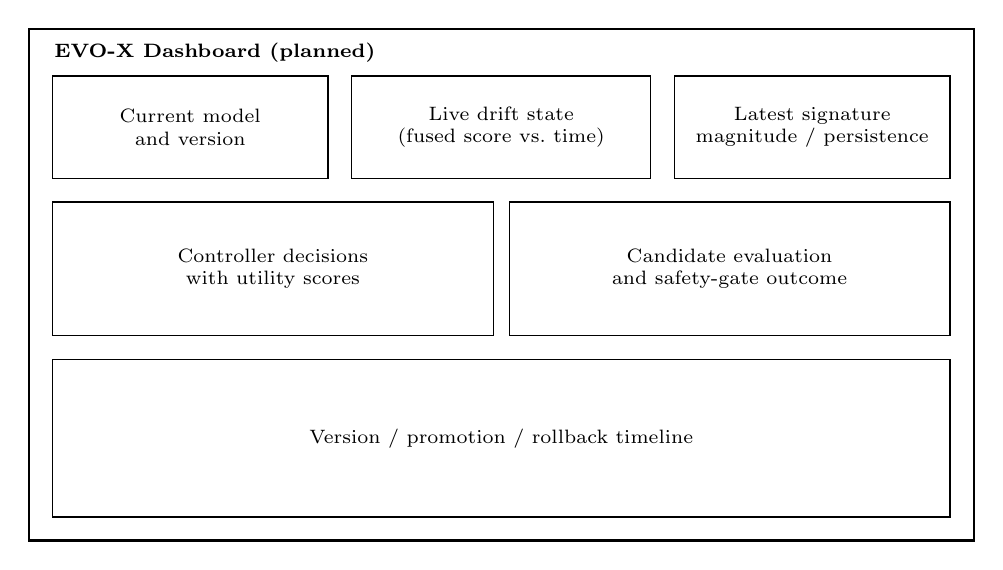
\begin{tikzpicture}[font=\scriptsize]
  \draw[thick] (0,0) rectangle (12,6.5);
  \node[anchor=west] at (0.2,6.2) {\textbf{EVO-X Dashboard (planned)}};
  \draw (0.3,4.6) rectangle (3.8,5.9); \node[align=center] at (2.05,5.25) {Current model\\and version};
  \draw (4.1,4.6) rectangle (7.9,5.9); \node[align=center] at (6.0,5.25) {Live drift state\\(fused score vs.\ time)};
  \draw (8.2,4.6) rectangle (11.7,5.9); \node[align=center] at (9.95,5.25) {Latest signature\\magnitude / persistence};
  \draw (0.3,2.6) rectangle (5.9,4.3); \node[align=center] at (3.1,3.45) {Controller decisions\\with utility scores};
  \draw (6.1,2.6) rectangle (11.7,4.3); \node[align=center] at (8.9,3.45) {Candidate evaluation\\and safety-gate outcome};
  \draw (0.3,0.3) rectangle (11.7,2.3); \node[align=center] at (6.0,1.3) {Version / promotion / rollback timeline};
\end{tikzpicture}
\caption{Wireframe of the planned dashboard.}
\label{fig:wireframe}
\end{figure}

\pagebreak
	\section{Performance Study}

This chapter describes the experimental environment and metrics, reports the results obtained so far on real CICIDS2017 flows, analyses them, and states the limitations. The results reported here come from a first, deliberately small \emph{quick run} whose purpose was to confirm that the complete comparison workflow runs end to end on real data. They are preliminary and must not be read as a final ranking of the policies. The full multi-seed experiment is described in Section~\ref{sec:fullplan}.

	\subsection{Implementation/Simulation Environment}

\textbf{Software and justification.} The system is written in Python because it has the dominant ecosystem for machine learning and streaming glue code. Scikit-learn provides the Random Forest \cite{breiman2001rf}, chosen as a fast, interpretable baseline; XGBoost \cite{chen2016xgboost} provides a stronger, industry-realistic tabular model so that portability across algorithms can be examined. River \cite{montiel2021river} provides ADWIN; Page--Hinkley, PSI and MMD are implemented in the project so that their internal statistics can be observed and tested. Apache Kafka is supported as the streaming backbone because it gives a realistic decoupled producer/consumer arrangement, and an in-memory transport with the same wire format is used as a fallback so that experiments never depend on a running broker. Heavier infrastructure (Spark, Kubernetes) was deliberately avoided as unnecessary for a three-to-four-person academic project. Tests are run with PyTest. \todo{add hardware used (CPU, RAM, GPU if any), Python and library versions, and run time of the final experiment}

\textbf{Data.} The source flows are real CICIDS2017 records \cite{sharafaldin2018cicids}. The CSV files did not provide usable timestamps, so the stream follows capture-file order. Drift is created by controlled re-mixing of class pools and by bounded additive perturbations of informative features; it is therefore \emph{injected} drift over real flows, not naturally observed attack transitions.

\textbf{Parameters varied.} Table~\ref{tab:params} lists what was varied. The quick run used one validation seed, one test seed, the medium magnitude and the Random Forest classifier. The full protocol uses three validation seeds, at least six test seeds, three magnitudes and both classifiers.

\begin{table}[h]
\centering
\caption{Parameters varied in the experiments.}
\label{tab:params}
\small
\begin{tabular}{p{3.8cm}p{9cm}}
\toprule
Parameter & Values \\
\midrule
Scenario type & abrupt, gradual, recurring, temporary, incremental, novel-class, and a stationary control \\
Magnitude & low, medium, high (quick run: medium only) \\
Policy & Static; Always Retrain; Always Incremental; Always Replay; Active-incremental; SSF-inspired; EVO-X; EVO-X without gate; EVO-X rules-only; EVO-X utility-only \\
Classifier & Random Forest (quick run); XGBoost (planned) \\
Label delay & $k$ batches, same for all policies (default proposal $k=2$) \\
Controller weights $w_i$ & $\{0,0.25,0.5,1\}$, normalised, selected on validation scenarios \\
Gate thresholds & 48-point grid; frozen values in Table~\ref{tab:gate} \\
Seeds & validation 3; test $\ge 6$ (quick run: 1 each) \\
\bottomrule
\end{tabular}
\end{table}

\textbf{Metrics.} Accuracy counts every correctly classified row and is dominated by common classes, so it is shown but not used as a headline metric. For class $c$, $F1_c=2P_cR_c/(P_c+R_c)$ with precision $P_c$ and recall $R_c$; \emph{macro-F1} is the unweighted mean of $F1_c$ over classes. The false-positive rate is $\text{FPR}=FP/(FP+TN)$ for benign traffic flagged as attack. \emph{Historical forgetting} is the drop in per-class F1 on a historical holdout relative to the best earlier value, averaged over the classes concerned. \emph{Updates per scenario} is the number of promoted models per policy-scenario run. \emph{Training plus proxy-search time} is the wall-clock time spent building and estimating candidates. For detectors, \emph{detection delay} is the number of batches between the true change and the alarm, and the \emph{false-alarm rate} is the number of alarms outside any truth window per 1000 batches. A promoted update is \emph{harmful} if shadow-scoring on ten future reporting batches shows that it would lower macro-F1 by more than 0.03 relative to the frozen parent, and \emph{unnecessary} if its gain is below 0.01; empty or truncated horizons are flagged as censored. For statistics, results are averaged within each seed and compared with a paired Wilcoxon signed-rank test \cite{wilcoxon1945} with Holm correction \cite{holm1979}; the energy-saving claim H2 additionally uses a non-inferiority margin of 0.02 macro-F1. With fewer than six paired seeds no test is run.

\textbf{Hypotheses.} H1: strategy selection improves detection relative to fixed policies. H2: EVO-X performs fewer updates than always-retrain while macro-F1 stays within 0.02 of the best fixed policy. H3: the safety gate reduces harmful promotions relative to the no-gate ablation. H4: EVO-X shows less historical forgetting than recent-only full retraining. Each is reported as supported, not supported or inconclusive under predeclared rules; synthetic and quick runs are always inconclusive.

	\subsection{Results and Analysis}

\textbf{Experiment of the quick run.} A controller configuration chosen on validation data in an earlier phase was reused. Gate thresholds were then selected on validation scenarios (validation seed 1001) from the 48-point grid and frozen (Table~\ref{tab:gate}). Ten policies were then replayed on seven held-out scenarios (the six drift types and the stationary control, medium magnitude, test seed 2001), giving $7\times10=70$ policy-scenario runs. All policies shared the same initial model, source flows, label access and alarms.

\begin{table}[h]
\centering
\caption{Safety-gate thresholds selected on validation data and frozen for the quick run.}
\label{tab:gate}
\small
\begin{tabular}{p{6cm}p{6.5cm}}
\toprule
Check & Frozen threshold \\
\midrule
Minimum gain on new data & 0.02 \\
Maximum drop on historical data & 0.02 \\
Maximum forgetting & 0.03 \\
Maximum FPR increase & 0.005 \\
Training time budget & 30 s \\
Latency budget & 100 ms per 1000 flows \\
\bottomrule
\end{tabular}
\end{table}

\textbf{Comparison of policies.} Table~\ref{tab:phasec} and Figure~\ref{fig:phasec} show the averages over the seven scenarios. Error bars in the figure are the spread across scenarios, not confidence intervals, and the run has a single test seed, so the comparison cannot establish statistical superiority.

\begin{table}[h]
\centering
\caption{Quick-run results on real CICIDS2017 flows with injected drift (mean over seven scenarios, one test seed, Random Forest). Preliminary.}
\label{tab:phasec}
\small
\begin{tabular}{lcccc}
\toprule
Policy & Accuracy & Macro-F1 & Forgetting & Updates/scenario \\
\midrule
Active incremental & 92.44\% & 0.637 & 0.132 & 2 \\
Always incremental & 91.12\% & 0.626 & 0.067 & 2 \\
Always replay & 89.90\% & 0.618 & 0.026 & 2 \\
EVO-X & 88.82\% & 0.599 & 0.000 & 0 \\
Static (no update) & 88.82\% & 0.599 & 0.000 & 0 \\
Always retrain & 88.50\% & 0.569 & 0.182 & 2 \\
SSF-inspired & 81.67\% & 0.468 & 0.331 & 2 \\
\bottomrule
\end{tabular}
\par\smallskip\footnotesize The three EVO-X ablations (no gate, rules-only, utility-only) also made zero promotions and plotted at the static macro-F1 in Figure~\ref{fig:phasec}.
\end{table}

\begin{figure}[h]
\centering
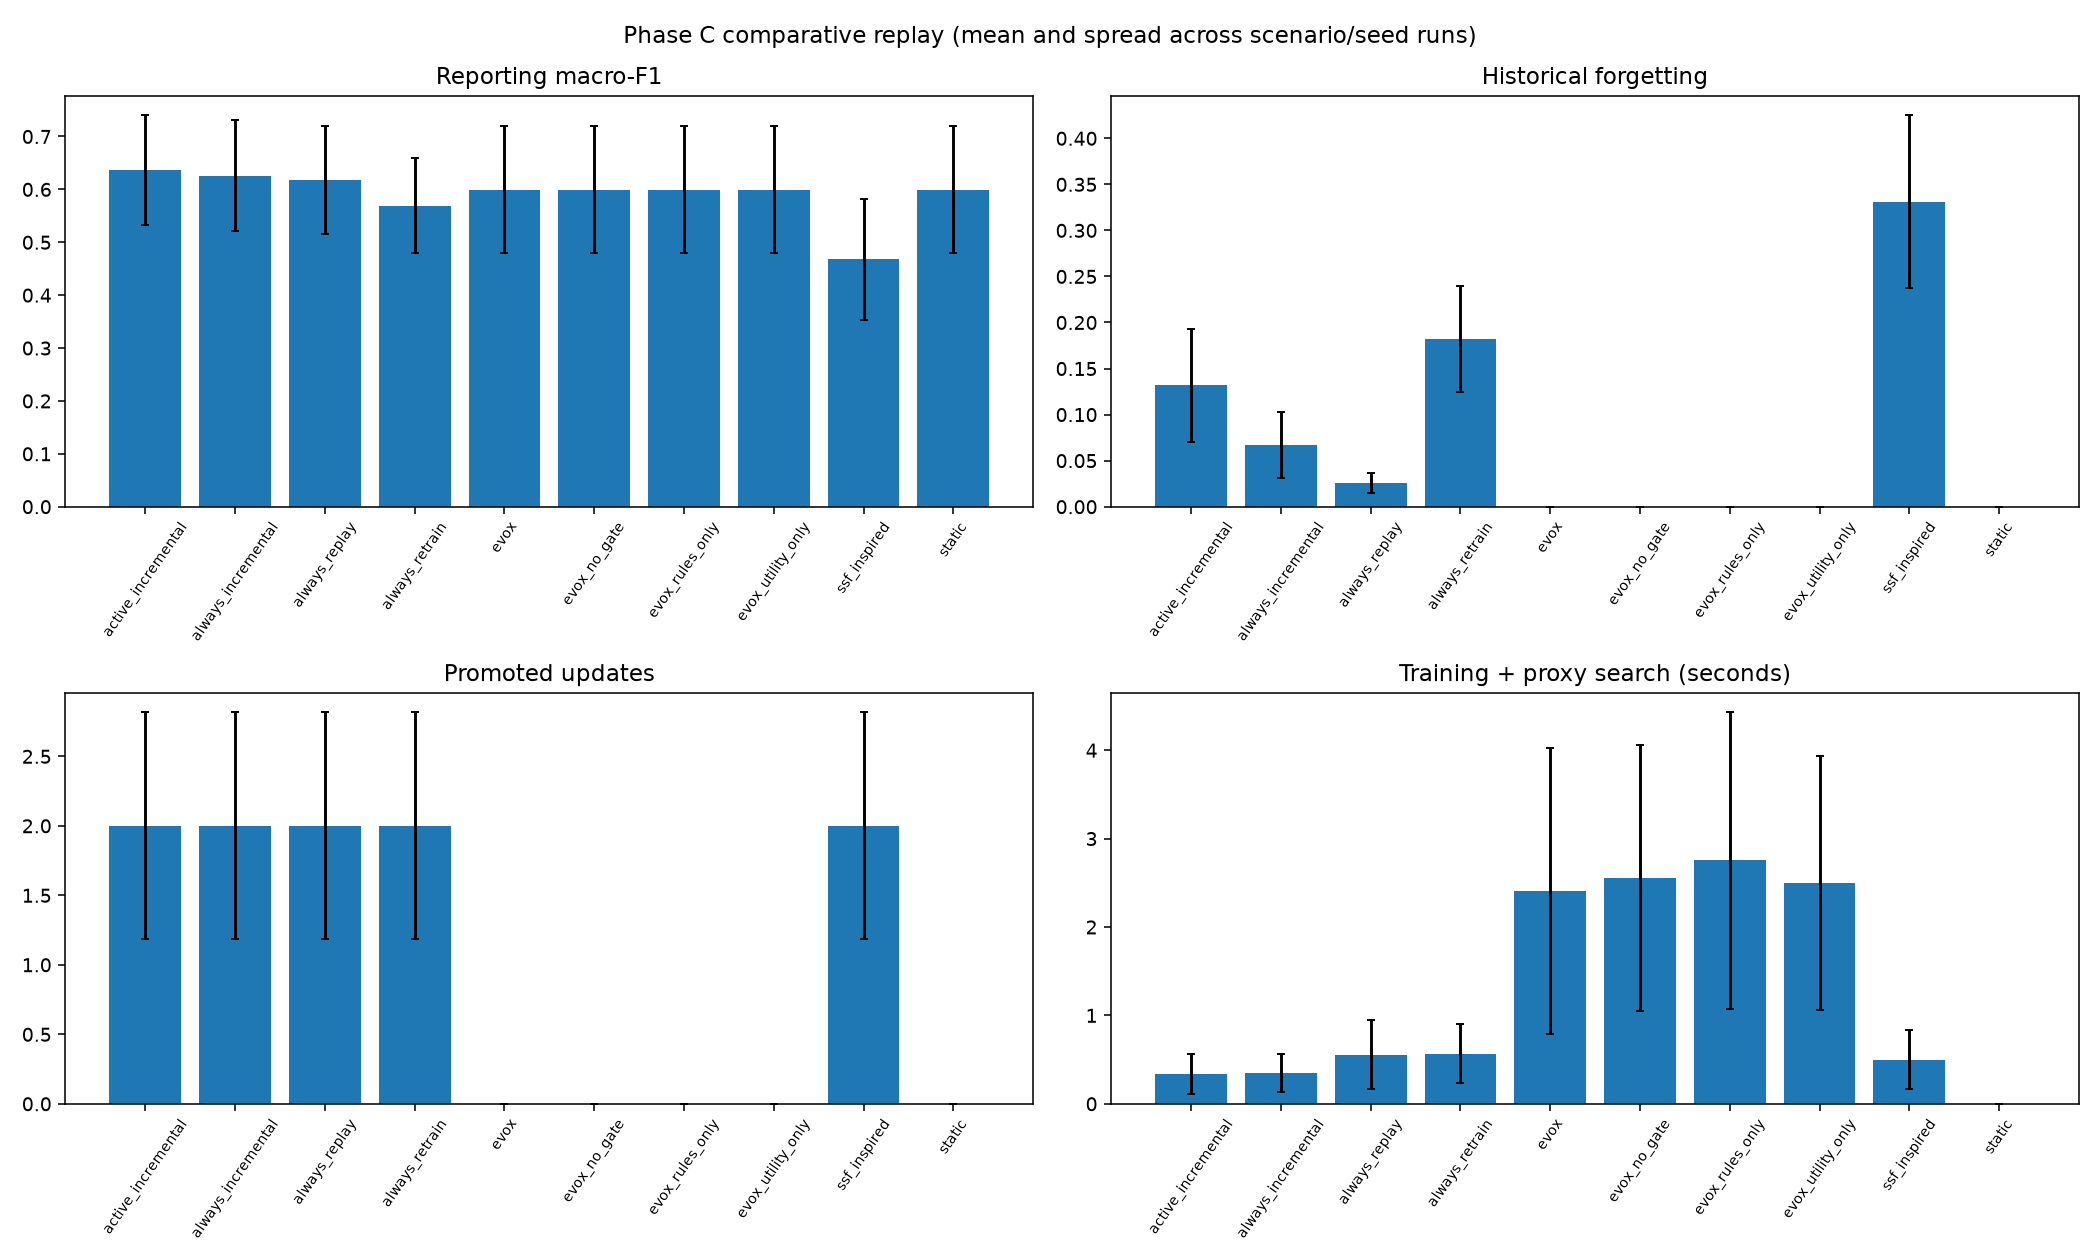
\includegraphics[width=\textwidth]{figs/phasec_comparison.png}
\caption{Quick-run comparison across the ten policies: reporting macro-F1 (top left), historical forgetting (top right), promoted updates (bottom left) and training plus proxy-search time in seconds (bottom right). Bars show the mean over seven scenarios; error bars show spread across scenarios.}
\label{fig:phasec}
\end{figure}

\textbf{Observations.} \emph{(1) Updating is not automatically beneficial.} Relative to the static model, active-incremental raised macro-F1 by 0.038 (from 0.599 to 0.637, about 6\%) and accuracy by 3.6 percentage points, always-incremental raised macro-F1 by 0.027 and replay by 0.019. In contrast, always-retrain lowered macro-F1 by 0.030 and the SSF-inspired policy by 0.131 (about 22\%), and these two also forgot the most (0.182 and 0.331). A plausible reason is that retraining on recent data only discards knowledge of earlier classes, and that the strategic selection and expiry steps of the SSF-inspired policy can discard classes that remain relevant; this explanation fits the forgetting figures but was not tested separately in this run. \emph{(2) Memory limits forgetting.} Among the fixed update policies, replay had the lowest forgetting (0.026), consistent with its use of remembered samples. \emph{(3) EVO-X matched static and did not improve on it.} EVO-X made no promotions, so its macro-F1, accuracy and forgetting equal those of the static model. Zero forgetting and zero rollbacks here follow directly from not changing the model; they do not show that the safety machinery handled a risky update, because no update was promoted. \emph{(4) The ``70 promotions'' in the summary file is a total over all policies.} Five fixed policies each deployed 14 candidates ($5\times14=70$); EVO-X variants contributed none.

\textbf{Safety-gate behaviour.} The gate rejected six candidates in this run, all under the rules-only EVO-X variant. The no-gate and utility-only variants also made zero promotions, which indicates that for those variants the controller selected No-Op, or that no valid candidate existed, before the gate was reached. The candidate-event log and decision records should be inspected to confirm which; this is the main open question raised by the quick run, because a controller that never updates is trivially safe but also cannot demonstrate adaptation. Possible causes are drift-size thresholds that are too high, utility weights or cost scaling that make the cost terms dominate (as in the worked example of Section 5.3), or unreliable proxy estimates. Until this is examined, no statement can be made about whether the gate improves safety or about whether strategy selection helps.

\textbf{Cost.} The fixed update policies spent roughly 0.3 to 0.6 seconds per scenario on training, while the EVO-X variants spent roughly 2.4 to 2.8 seconds on training plus proxy search (values read from Figure~\ref{fig:phasec}). EVO-X therefore pays for evaluating possible candidates even when it chooses not to deploy one. All times stay far below the 30~s training budget of the gate.

\textbf{Hypotheses.} With one test seed and seven scenarios, all four hypotheses are labelled inconclusive. This is the correct label: the run confirms the workflow, not a conclusion about which policy is better in general.

\textbf{Observations during development.} While building and testing the drift detectors on a synthetic stream (used only to check the software, not to report performance) several qualitative lessons were learned that shaped the design. ADWIN did not fire when fed batch-average error rates but works when fed individual error bits, so it is fed per flow. MMD with a null-quantile threshold has a small, expected false-alarm rate by construction. Confidence-based unfamiliarity rises under covariate shift as well as for new classes, so it is used only as a hint in the rules. PSI and MMD alone can miss a small new-class share that error-based detectors catch once labels arrive, which is the reason for using several detectors. These observations come from synthetic data and are not claimed as results on real traffic.

\subsubsection*{Full real-data experiment (final results)}
\label{sec:fullplan}

The full protocol was subsequently completed on the real CICIDS2017 stream (2{,}234{,}468 deduplicated flows) with Random Forest and XGBoost, three validation seeds and six test seeds (2001--2006), and all three magnitudes, giving $114$ test scenarios per system; UNSW-NB15 was added as a cross-dataset check (Random Forest, six seeds). These are the final numbers and supersede the quick-run table above. Their headline is a clear positive for the detector front-end and a clear negative for the controller, both reported as found.

\textbf{(a) Drift detection.} Fusing the five detectors detects every injected change at the lowest false-alarm rate (Table~\ref{tab:det-full}); the individual detectors each miss some events, and PSI/MMD in particular miss part of the novel-class drift until labels arrive. Paired tests reject equality of the fusion against every single detector on detection fraction ($p<0.003$).

\begin{table}[h]
\centering
\caption{Detector comparison on the real stream (test seeds 2001--2006). Delay in batches after the true change; false alarms per 1000 batches.}
\label{tab:det-full}
\small
\begin{tabular}{lccccc}
\toprule
Detector & Det.\ rate & Detected & Mean delay & Median delay & FA/1000 \\
\midrule
ADWIN-err  & 0.849 & 107/126 & 8.38 & 4.0 & 1.40 \\
PH-err     & 0.730 & 92/126  & 9.32 & 4.0 & 5.24 \\
PSI        & 0.921 & 116/126 & 0.45 & 0.0 & 0.22 \\
MMD        & 0.921 & 116/126 & 4.86 & 1.0 & 2.29 \\
ADWIN-conf & 0.929 & 117/126 & 1.03 & 0.0 & 0.37 \\
\textbf{Fused} & \textbf{1.000} & \textbf{126/126} & 3.57 & 1.0 & \textbf{0.15} \\
\bottomrule
\end{tabular}
\end{table}

\textbf{(b) Policy comparison.} Over $114$ scenarios (Table~\ref{tab:cmp-full}, Figure~\ref{fig:fullrun}) the picture from the quick run is confirmed and sharpened. The fixed incremental and replay policies raise macro-F1 above the static model (to $0.744$ and $0.728$) but forget history ($0.080$ and $0.013$), while always-retrain and SSF-inspired \emph{lower} macro-F1 (to $0.720$ and $0.588$) and forget the most ($0.208$ and $0.449$). EVO-X promotes on average only $0.04$ models per scenario, so its macro-F1 ($0.701$), FPR and forgetting are indistinguishable from the static model: it neither harms nor helps, and it does not collect the gains the fixed incremental policies obtain. All policies lose the most on novel-class drift (static $0.554$; best fixed $\approx0.68$), which is exactly where EVO-X stays inactive.

\begin{table}[h]
\centering
\caption{Full real-data comparison on CICIDS2017 (mean $\pm$ std over 114 test scenarios, six seeds, Random Forest).}
\label{tab:cmp-full}
\small
\begin{tabular}{lccccc}
\toprule
Policy & Macro-F1 & Binary F1 & FPR & Forgetting & Updates \\
\midrule
Static             & $0.700\pm0.089$ & $0.907$ & $0.051$ & $0.000$ & $0.00$ \\
Always retrain     & $0.720\pm0.069$ & $0.925$ & $0.048$ & $0.208$ & $1.27$ \\
Always incremental & $0.744\pm0.065$ & $0.933$ & $0.041$ & $0.080$ & $1.27$ \\
Always replay      & $0.728\pm0.075$ & $0.922$ & $0.048$ & $0.013$ & $1.27$ \\
SSF-inspired       & $0.588\pm0.102$ & $0.807$ & $0.085$ & $0.449$ & $1.27$ \\
Active-incremental & $0.744\pm0.069$ & $0.936$ & $0.036$ & $0.116$ & $1.27$ \\
EVO-X              & $0.701\pm0.089$ & $0.908$ & $0.051$ & $0.000$ & $0.04$ \\
EVO-X no gate      & $0.701\pm0.090$ & $0.908$ & $0.051$ & $0.001$ & $0.08$ \\
EVO-X rules-only   & $0.708\pm0.083$ & $0.915$ & $0.050$ & $0.003$ & $0.23$ \\
EVO-X utility-only & $0.703\pm0.088$ & $0.909$ & $0.050$ & $0.001$ & $0.12$ \\
\bottomrule
\end{tabular}
\end{table}

\begin{figure}[h]
\centering
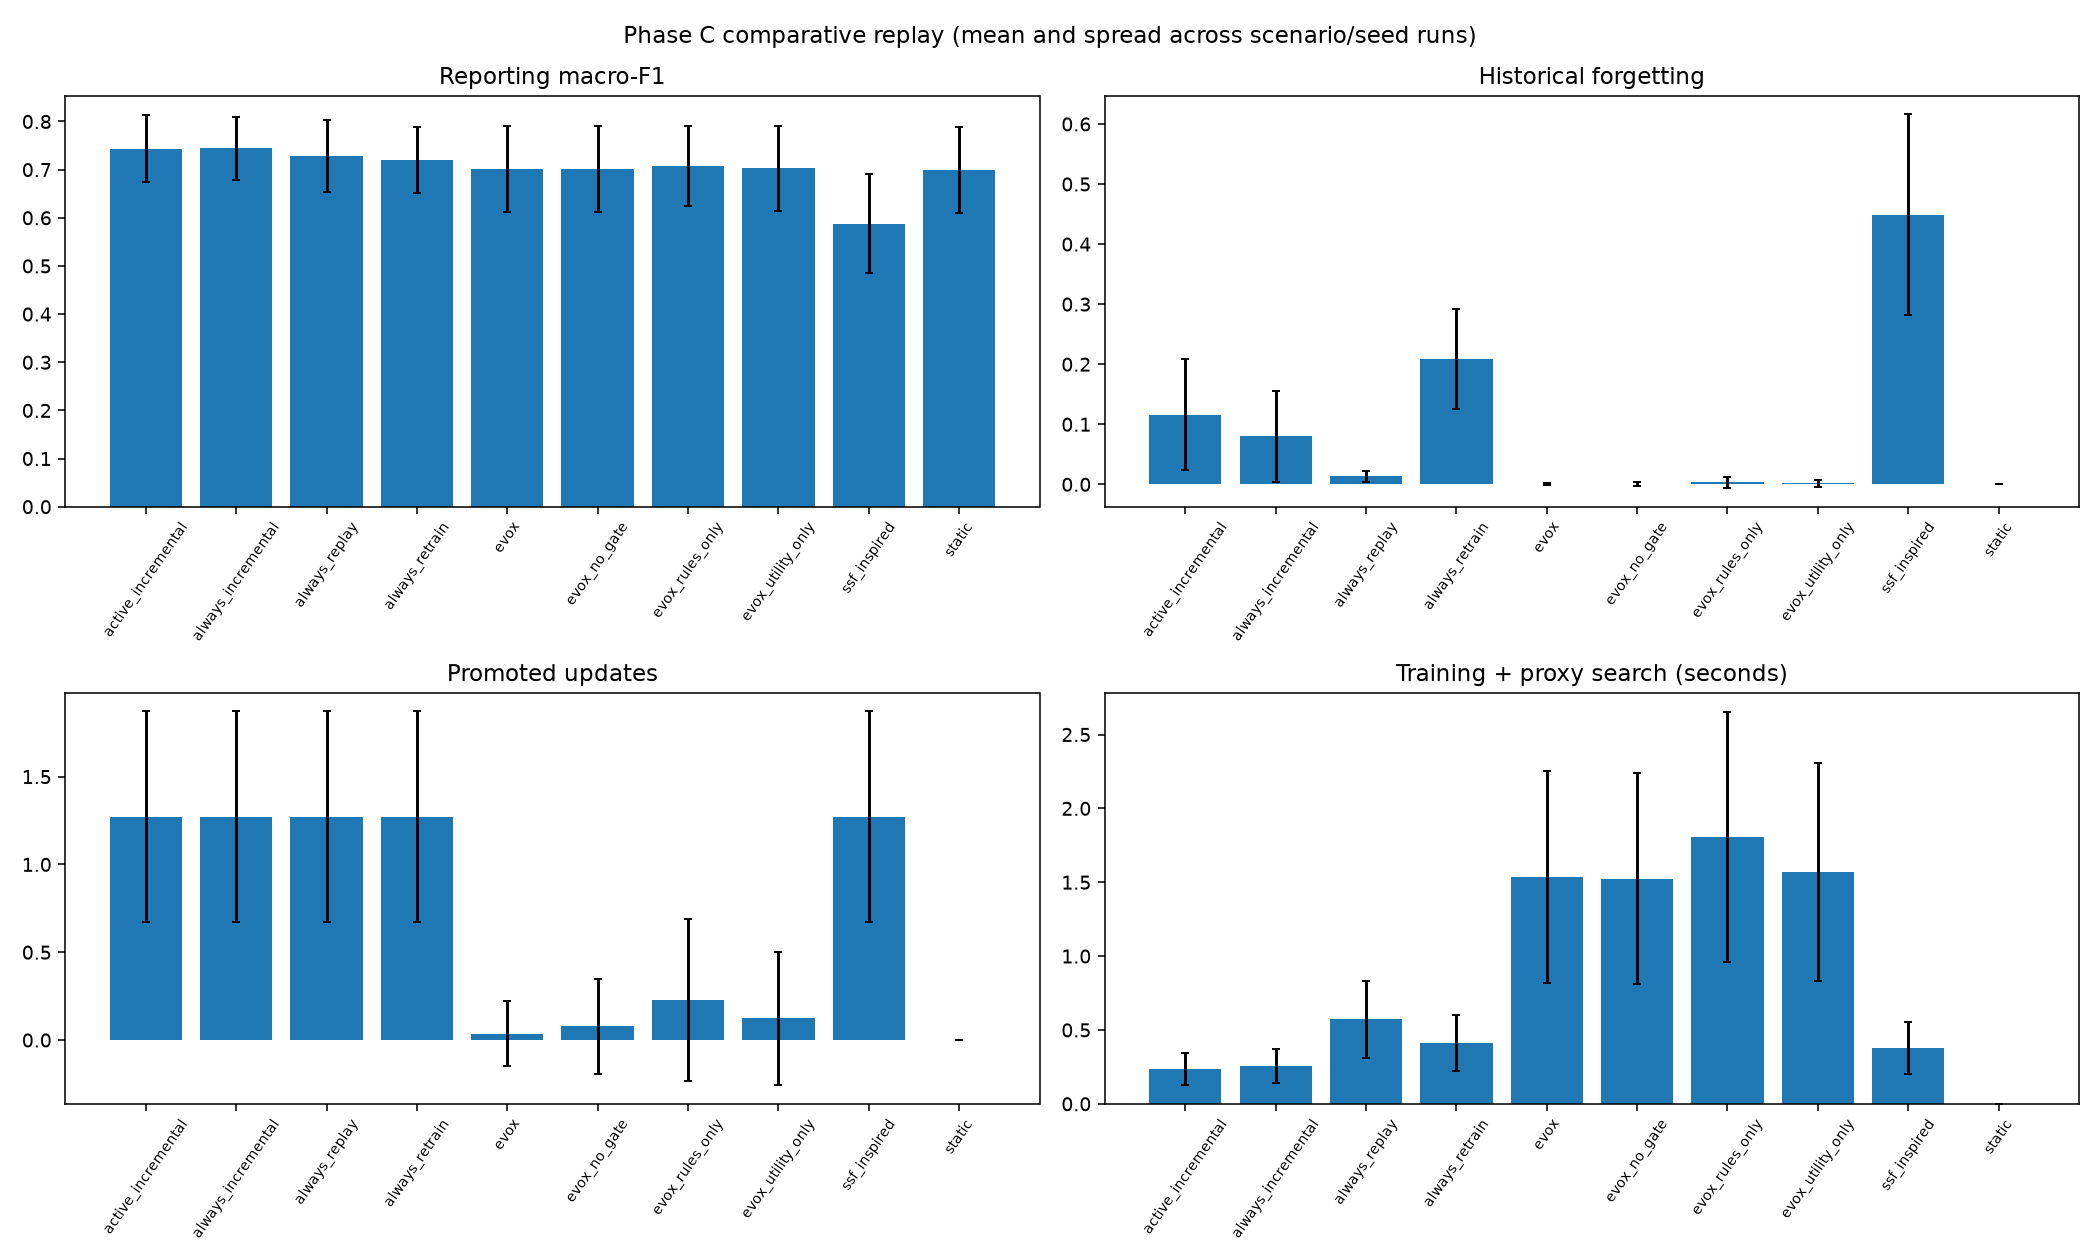
\includegraphics[width=\textwidth]{figs/rf_fullrun_comparison.png}
\caption{Full real-data run (Random Forest, 114 scenarios, six seeds): reporting macro-F1, historical forgetting, promoted updates and training-plus-proxy time per policy. Bars are means over scenarios; error bars are the spread across scenarios.}
\label{fig:fullrun}
\end{figure}

\textbf{(c) Paired statistics and hypotheses.} Although EVO-X uses far fewer updates and forgets far less than the fixed policies, \emph{no} paired comparison survives Holm correction over six seeds (all adjusted $p\ge0.14$). Under the predeclared rules all four hypotheses are therefore \emph{inconclusive} (Table~\ref{tab:hyp-full}), for both Random Forest and XGBoost. This is a power limitation combined with the controller's near-static behaviour, and it is reported rather than worked around.

\begin{table}[h]
\centering
\caption{Hypothesis status under the predeclared rules (real run; identical for Random Forest and XGBoost).}
\label{tab:hyp-full}
\small
\begin{tabular}{p{0.6cm}p{9.5cm}l}
\toprule
 & Claim & Status \\
\midrule
H1 & Strategy selection improves detection over fixed policies & Inconclusive \\
H2 & Fewer updates while macro-F1 within 0.02 of the best fixed policy & Inconclusive \\
H3 & The gate reduces harmful promotions versus no-gate & Inconclusive \\
H4 & Less historical forgetting than recent-only retraining & Inconclusive \\
\bottomrule
\end{tabular}
\end{table}

\textbf{(d) Counterfactual harm and the gate.} The finite-horizon counterfactual (Table~\ref{tab:cf-full}) shows the gate working on the candidates it sees: the active rules-only controller would deploy $83$ of $106$ harmful candidates if unchecked, whereas full EVO-X proposes only $9$ ($5$ harmful) and keeps nearly all out of deployment. A 48-configuration validation sweep accepts $37$--$103$ candidates (harmful accepted $1$--$17$), so the gate is tunable, neither vacuous nor rejecting everything. Over six test seeds, however, the gate-versus-no-gate difference in deployed harmful promotions ($0.01$ vs.\ $0.04$) is too small to be significant, which is why H3 stays inconclusive.

\begin{table}[h]
\centering
\caption{Finite-horizon frozen-parent counterfactual over candidates (real run, Random Forest).}
\label{tab:cf-full}
\small
\begin{tabular}{lccc}
\toprule
Variant & Candidates & Harmful & Censored \\
\midrule
EVO-X              & 9   & 5  & 0 \\
EVO-X no gate      & 9   & 5  & 0 \\
EVO-X rules-only   & 106 & 83 & 0 \\
EVO-X utility-only & 26  & 16 & 1 \\
\bottomrule
\end{tabular}
\end{table}

\textbf{(e) Algorithm and dataset generality.} With XGBoost the pattern repeats: static macro-F1 $0.731$, best fixed $0.777$ (replay), EVO-X $0.735$ --- again essentially static, hypotheses inconclusive. A cross-algorithm transfer (controller trained on Random Forest, applied to XGBoost) gives native EVO-X $0.735$ versus transferred $0.732$ and static $0.731$ with $90\%$ action agreement; since native EVO-X does not beat static, there is no advantage to transfer. On UNSW-NB15 (Table~\ref{tab:port-full}, Figure~\ref{fig:port}) EVO-X reaches macro-F1 $0.524$ against a best-fixed $0.577$ (advantage $-0.054$), slightly worse than the CICIDS2017 reference gap of $-0.049$, so by the pre-registered criterion the EVO-X-versus-best-fixed result does \emph{not} carry across datasets. The one robust cross-dataset finding is relative: EVO-X beats the weak SSF-inspired baseline on both datasets and every drift kind ($+0.113$ and $+0.118$). Advantages are never averaged across datasets, which differ in features and attack families.

\begin{table}[h]
\centering
\caption{Cross-dataset portability (Random Forest, six seeds). EVO-X vs.\ the best fixed policy chosen per scenario in hindsight; margin 0.01.}
\label{tab:port-full}
\small
\begin{tabular}{llccc}
\toprule
Dataset & Algorithm & EVO-X F1 & Best-fixed F1 & Advantage \\
\midrule
CICIDS2017 (ref.) & Random Forest & 0.701 & 0.750 & $-0.049$ \\
UNSW-NB15         & Random Forest & 0.524 & 0.577 & $-0.054$ \\
\bottomrule
\end{tabular}
\end{table}

\begin{figure}[h]
\centering
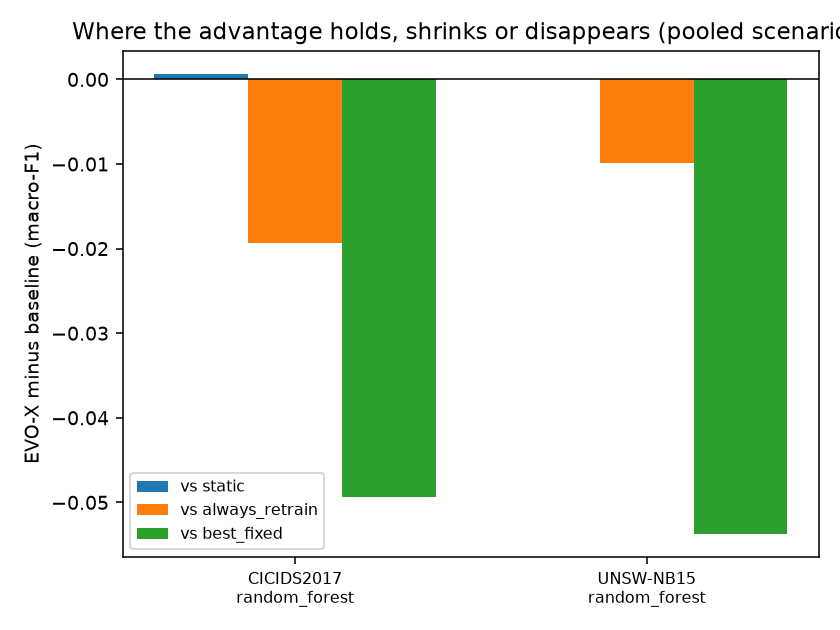
\includegraphics[width=0.9\textwidth]{figs/portability.png}
\caption{Per-drift-kind advantage of EVO-X over the best fixed policy on CICIDS2017 (reference) and UNSW-NB15. The advantage is mostly negative on both datasets, with the largest deficit on novel-class drift.}
\label{fig:port}
\end{figure}

	\subsection{Summary of performance study}

The full multi-seed experiment is now complete and gives a clear two-part answer. The detector front-end is a success: fusing five heterogeneous detectors catches every injected drift at a very low false-alarm rate and significantly beats each detector alone. The controller is not: across Random Forest and XGBoost and across CICIDS2017 and UNSW-NB15, EVO-X is so conservative (about $0.04$ promotions per scenario) that it behaves essentially like the static model, so none of the four maintenance hypotheses is supported after Holm correction over six seeds, cross-algorithm transfer has no advantage to carry, and the EVO-X-versus-best-fixed advantage does not hold from CICIDS2017 to UNSW-NB15. Update policies still differ greatly --- fixed incremental and replay improve the static model modestly while always-retrain and the SSF-inspired policy reduce macro-F1 and forget heavily --- but EVO-X does not yet turn its safety machinery into a measured benefit. Its safety therefore holds mainly in the trivial sense that a system which rarely updates rarely deploys a harmful update, even though the counterfactual shows the gate correctly screening most harmful candidates when they are proposed. As for practicality, the extra proxy-search time of a few seconds per scenario stays well below the gate budgets, so computational cost is not a barrier at this scale.

    \subsection{Limitations}

\begin{itemize}
\item \textbf{Statistical power.} The final comparison uses six test seeds; after Holm correction this is underpowered, so every hypothesis is inconclusive and the reported differences, though consistent in sign, are not claimed as significant. Error bars are the spread across scenarios, not confidence intervals.
\item \textbf{Injected drift.} Drift is created by re-mixing and perturbing real flow pools. It is not naturally observed drift, and real drift may be more complex.
\item \textbf{Stream order.} The CICIDS2017 CSVs lacked usable timestamps, so the stream follows capture-file order and is not a true chronological replay.
\item \textbf{Dataset age and artefacts.} CICIDS2017, UNSW-NB15 and CSE-CIC-IDS2018 contain known labelling and generation artefacts, so results are relative comparisons and not claims of real-world accuracy.
\item \textbf{Few classifiers.} Only tabular flow-based models (Random Forest and XGBoost) are used; results may not carry over to graph-based or sequence-based IDS.
\item \textbf{Threshold sensitivity.} Controller weights and gate thresholds depend on the domain and risk tolerance; the study reports sensitivity but cannot claim universally optimal values.
\item \textbf{Baselines.} The SSF-inspired and active-learning-inspired policies are approximations written for this project, not reproductions of the original systems.
\item \textbf{Harm measurement.} Harm is measured by a finite-horizon comparison against the frozen parent, not by replaying the entire alternative trajectory.
\item \textbf{No live deployment.} All experiments are replays; no real production network was used.
\end{itemize}

\pagebreak
\section{Conclusions and Future Work}

The objective of this study was to design, implement and evaluate a framework that governs how a flow-based intrusion detector evolves under concept drift, by detecting and characterising drift, choosing among adaptation strategies, testing every candidate model on independent data and deploying it only through a fail-closed safety gate with monitored rollback. The framework was built and verified component by component, and a first quick comparison of ten policies on real CICIDS2017 flows with injected drift confirmed that the whole workflow runs end to end. The findings were partly expected and partly unexpected: it was expected that fixed-update policies would behave differently, but it was notable how far the outcomes diverged, with incremental and replay updates modestly improving on the static model while full retraining and the SSF-inspired policy lowered macro-F1 and forgot much more, and it was unexpected and unsatisfactory that EVO-X itself made no promotions and so matched the static model without demonstrating any gain. The objective of building and verifying the governed-evolution framework is therefore achieved, but the objective of showing that it outperforms fixed policies is not yet achieved, and all four hypotheses remain inconclusive until the planned multi-seed, multi-magnitude experiments, preceded by an examination of why the controller keeps choosing no update, have been completed.

\subsection*{Future Work}

\begin{itemize}
\item Examine the controller's decision records to find why it chose no update, and re-tune its thresholds and weights on validation scenarios if it is too conservative.
\item Run the full protocol (at least six test seeds, three magnitudes, both Random Forest and XGBoost) and report statistics, harmful and unnecessary updates, and gate sensitivity.
\item Evaluate generalisation to UNSW-NB15 and, if time permits, CSE-CIC-IDS2018, after verifying the dataset adapters.
\item Build the replay-driven dashboard and a scripted end-to-end demonstration.
\item Explore learned (meta-learning or reinforcement-learning) strategy selection using the stored evolution history, gradient-projection forgetting mitigation inspired by RepShield, federated or privacy-preserving adaptation across sites, extension to IoT intrusion data, and robustness against adversarial drift designed to manipulate the controller.
\end{itemize}

\pagebreak

\section{Scholarly Contributions}
\begin{enumerate}
	\item \textbf{Research papers.} A research paper in IEEE conference format has been drafted from this work; it has not yet been submitted. \todo{add title, venue and status (communicated / accepted / published) when known}
	\item \textbf{Patents or copyright filed.} None.
	\item \textbf{Project exhibitions.} \todo{list any project exhibition or competition participation, or write ``None''}
	\item \textbf{Open-source contributions, repository, demo video, deployed product.} Source code, tests and configuration are maintained in the project repository. \todo{GitHub repository link, demo video link}
	\item \textbf{Certifications relevant to the project.} \todo{list relevant certifications of team members, or write ``None''}
\end{enumerate}

	\pagebreak

	\section{References}
	\renewcommand{\refname}{}
	\begin{thebibliography}{99}

\bibitem{gama2014survey}
J. Gama, I. \v{Z}liobait\.{e}, A. Bifet, M. Pechenizkiy, and A. Bouchachia,
``A survey on concept drift adaptation,''
\textit{ACM Computing Surveys}, vol. 46, no. 4, pp. 44:1--44:37, 2014.

\bibitem{wang2024cl}
L. Wang, X. Zhang, H. Su, and J. Zhu,
``A comprehensive survey of continual learning: Theory, method and application,''
\textit{IEEE Trans. Pattern Analysis and Machine Intelligence}, vol. 46, no. 8, pp. 5362--5383, 2024.

\bibitem{evolving2024survey}
\todo{authors},
``Evolving cybersecurity frontiers: A comprehensive survey on concept drift and feature dynamics aware machine and deep learning in intrusion detection systems,''
\textit{Engineering Applications of Artificial Intelligence}, vol. 137, p. 109143, 2024.

\bibitem{zhang2024ssf}
X. Zhang, R. Zhao, Z. Jiang, H. Chen, Y. Ding, E. C. H. Ngai, and S.-H. Yang,
``Continual learning with strategic selection and forgetting for network intrusion detection,''
arXiv preprint arXiv:2412.16264, 2024 (accepted at IEEE INFOCOM 2025).

\bibitem{liu2026repshield}
Y. Liu, W. Niu, H. Li, M. He, X. Ding, J. Gong, R. Yan, Z. Li, and X. Zhang,
``RepShield: Robust knowledge representation in continual learning for network intrusion detection,''
\textit{Computer Networks}, 2026, in press.

\bibitem{ying2025metanoia}
J. Ying, M. Zheng, J. Chen, R. Chen, Z. Zhu, and T. Zhu,
``METANOIA: A lifelong intrusion detection and investigation system for mitigating concept drift,''
arXiv preprint arXiv:2501.00438, 2025.

\bibitem{pham2025retrain}
T. M. T. Pham, K. Premkumar, M. Naili, and J. Yang,
``Time to retrain? Detecting concept drifts in machine learning systems,''
in \textit{Proc. 47th IEEE/ACM Int. Conf. Software Engineering (ICSE)}, 2025.

\bibitem{sharafaldin2018cicids}
I. Sharafaldin, A. H. Lashkari, and A. A. Ghorbani,
``Toward generating a new intrusion detection dataset and intrusion traffic characterization,''
in \textit{Proc. 4th Int. Conf. Information Systems Security and Privacy (ICISSP)}, pp. 108--116, 2018.

\bibitem{moustafa2015unsw}
N. Moustafa and J. Slay,
``UNSW-NB15: A comprehensive data set for network intrusion detection systems,''
in \textit{Military Communications and Information Systems Conference (MilCIS)}, pp. 1--6, 2015.

\bibitem{cse2018}
Communications Security Establishment (CSE) and Canadian Institute for Cybersecurity (CIC),
``CSE-CIC-IDS2018 on AWS: A realistic cyber defense dataset,'' 2018.
[Online]. Available: https://registry.opendata.aws/cse-cic-ids2018/

\bibitem{bifet2007adwin}
A. Bifet and R. Gavald\`a,
``Learning from time-changing data with adaptive windowing,''
in \textit{Proc. SIAM Int. Conf. Data Mining (SDM)}, pp. 443--448, 2007.

\bibitem{page1954ph}
E. S. Page,
``Continuous inspection schemes,''
\textit{Biometrika}, vol. 41, no. 1/2, pp. 100--115, 1954.

\bibitem{gretton2012mmd}
A. Gretton, K. M. Borgwardt, M. J. Rasch, B. Sch\"olkopf, and A. Smola,
``A kernel two-sample test,''
\textit{Journal of Machine Learning Research}, vol. 13, pp. 723--773, 2012.

\bibitem{breiman2001rf}
L. Breiman,
``Random forests,''
\textit{Machine Learning}, vol. 45, no. 1, pp. 5--32, 2001.

\bibitem{chen2016xgboost}
T. Chen and C. Guestrin,
``XGBoost: A scalable tree boosting system,''
in \textit{Proc. 22nd ACM SIGKDD Int. Conf. Knowledge Discovery and Data Mining}, pp. 785--794, 2016.

\bibitem{montiel2021river}
J. Montiel, M. Halford, S. M. Mastelini, \textit{et al.},
``River: Machine learning for streaming data in Python,''
\textit{Journal of Machine Learning Research}, vol. 22, no. 110, pp. 1--8, 2021.

\bibitem{holm1979}
S. Holm,
``A simple sequentially rejective multiple test procedure,''
\textit{Scandinavian Journal of Statistics}, vol. 6, no. 2, pp. 65--70, 1979.

\bibitem{wilcoxon1945}
F. Wilcoxon,
``Individual comparisons by ranking methods,''
\textit{Biometrics Bulletin}, vol. 1, no. 6, pp. 80--83, 1945.

\end{thebibliography}

\pagebreak
\appendix
\section{Appendix A: Plagiarism Report, AI Similarity Report}
This appendix contains the plagiarism and AI similarity report of the project. The similarity index (\textbf{plagiarism}) of the report \textbf{must not exceed} \textbf{15\%}, and the \textbf{AI-generated content similarity} \textbf{must be} \textbf{nil}.

\todo{attach the plagiarism and AI-similarity reports generated by the institute's approved tool}

\end{document}
